\ifdefined\included
\else
\documentclass[french, a4paper, 11pt, twoside, pdftex]{StyleThese}
\usepackage{iflang}
\usepackage{bibentry}



%\usepackage[sectionbib]{chapterbib}          % Cross-reference package (Natural BiB)
%\usepackage{natbib}                  % Put References at the end of each chapter
%\usepackage{bibunits}
% Do not put 'sectionbib' option here.
% Sectionbib option in 'natbib' will do.


\usepackage{fancyhdr}                    % Fancy Header and Footer

\usepackage[utf8]{inputenc}
\usepackage[T1]{fontenc}
\usepackage[french]{babel} %
\usepackage{lmodern} \normalfont %to load T1lmr.fd 
\DeclareFontShape{T1}{cmr}{b}{sc} { <-> ssub * cmr/bx/sc }{}
%\hyphenation{gar}

\usepackage{amsmath,amssymb}             % AMS Math
\usepackage{nicefrac}
\usepackage{siunitx}					%% Unites Math SI

\usepackage{blindtext}

\usepackage{datetime}

\usepackage{lipsum} 

\usepackage[inline]{enumitem}

\usepackage{hhline}
%\usepackage[left=1.5in,right=1.3in,top=1.1in,bottom=1.1in]{geometry}
\usepackage[left=1.5in,right=1.3in,top=1.1in,bottom=1.1in,includefoot,includehead,headheight=13.6pt]{geometry}

%%\renewcommand{\baselinestretch}{1.05}

%%%%%%%% Multi-figures avec sub-captions
\usepackage{caption}
\usepackage{subcaption}

% Table of contents for each chapter

\usepackage[nottoc, notlof, notlot]{tocbibind}
\usepackage[nohints]{minitoc}
\setcounter{minitocdepth}{2}
\mtcindent=15pt
% Use \minitoc where to put a table of contents

\usepackage{aecompl}

%% Package cosmetic meilleur layout du texte en jouant sur le spacing par caractères
\usepackage[activate={true,nocompatibility},final,tracking=true,kerning=true,factor=1100,stretch=10,shrink=10]{microtype}
\usepackage[absolute,overlay]{textpos} 
\setlength{\TPHorizModule}{\paperwidth}\setlength{\TPVertModule}{\paperheight}
\sloppy

%%%%%%%%%%% JOLIS TABLEAUX
\usepackage{tabularx}		%\usepackage{tabular}
\usepackage{longtable}
\usepackage{multirow}
\newcommand{\mc}{\multicolumn} 
\newcommand{\mr}[2]{\multirow{#1}{*}{#2}} 	\newcommand{\mrQ}{\multirow{-4}{*}}
\usepackage{booktabs}

\usepackage[usenames,dvipsnames]{xcolor} 

\makeatletter
\newcommand{\ccolor}[3][]{%
	\kern-\fboxsep
	\if\relax\detokenize{#1}\relax
	\expandafter\@firstoftwo
	\else
	\expandafter\@secondoftwo
	\fi
	{\colorbox{#2}}%
	{\colorbox[#1]{#2}}%
	{#3}\kern-\fboxsep
}
\makeatother

%%%%% Insertion graphiques format PGF
\usepackage{pgfplots}
\pgfplotsset{width=\linewidth, compat=1.16}%, compat=1.17}
\usepackage{adjustbox}          %%% PERMET DE LES RECADRER + FACILEMENT


%%%%%%%%%% Bullets de listes sans saut de ligne %%%%%%%%%%
\usepackage{xparse}

\ExplSyntaxOn%
\seq_new:N \l_local_enum_seq

\newcommand{\storethestuff}[1]{%
  \seq_set_from_clist:Nn \l_local_enum_seq {#1}%
}

\newcommand{\dotheenumstuff}{%
\int_zero:N \l_tmpa_int
\seq_map_inline:Nn \l_local_enum_seq {%
    \int_incr:N \l_tmpa_int% Increase the counter
    \item ##1
    % Check whether the list has reached the end -- if so, use '.' instead of ','
    %\int_compare:nNnTF 
    % { \l_tmpa_int } < {\seq_count:N \l_local_enum_seq} 
    % {,} {.}
  }
}
\ExplSyntaxOff

\NewDocumentCommand{\linebullets}{+m}{%
  \storethestuff{#1}%
  \begin{enumerate*}[label={\alph*)},font={\bfseries},itemjoin={{, }}]
    \dotheenumstuff%
  \end{enumerate*}
}

\newcommand{\cmnt}[1]{}  %%%%% AJOUT DE COMMENTAIRE MULTILIGNES


%%%%%%%%%% ECRITURE CARACTERES DANS UN CERCLE %%%%%%%%%%
%\def\circleTxt[#1]{\raisebox{.5pt}{\textcircled{\raisebox{-1pt}{#1}}}}
\newcommand{\ctxt}[1]{\raisebox{.5pt}{\textcircled{\raisebox{-1.2pt}{#1}}}}
% Glossary / list of abbreviations

\usepackage[intoc]{nomencl}
\IfLanguageName{english}{%
\renewcommand{\nomname}{Glossary}
}{ %
\renewcommand{\nomname}{Liste des Abréviations}
}

\makenomenclature

% My pdf code

\usepackage{ifpdf}

\ifpdf
  \usepackage[pdftex]{graphicx}
  \DeclareGraphicsExtensions{.pdf,PDF,.png,PNG,.jpg,JPG}
  \usepackage[pagebackref,hyperindex=true]{hyperref} %% use \autoref{} instead of Table~\ref{}.
  \usepackage{tikz}
  \usetikzlibrary{arrows,shapes,calc}
\else
  \usepackage{graphicx}
  \DeclareGraphicsExtensions{.ps,.eps}
  \usepackage[a4paper,dvipdfm,pagebackref,hyperindex=true]{hyperref}
\fi

\graphicspath{{.}{schemas/}{graphiques/}{tables/}}

%% nicer backref links. NOTE: The flag ThesisInEnglish is used to define the
% language in the back references. Read more about it in These.tex

\IfLanguageName{english}{
\renewcommand*{\backref}[1]{}
\renewcommand*{\backrefalt}[4]{%
\ifcase #1 %
(Not cited.)%
\or
(Cited in page~#2.)%
\else
(Cited in pages~#2.)%
\fi}
\renewcommand*{\backrefsep}{, }
\renewcommand*{\backreftwosep}{ and~}
\renewcommand*{\backreflastsep}{ and~}
}{
\renewcommand*{\backref}[1]{}
\renewcommand*{\backrefalt}[4]{%
\ifcase #1 %
(Non cité.)%
\or
(Cité en page~#2.)%
\else
(Cité en pages~#2.)%
\fi}
\renewcommand*{\backrefsep}{, }
\renewcommand*{\backreftwosep}{ et~}
\renewcommand*{\backreflastsep}{ et~}
}

% Links in pdf
\usepackage{color}
\definecolor{linkcol}{rgb}{0,0,0.4} 
\definecolor{citecol}{rgb}{0.5,0,0} 
\definecolor{linkcol}{rgb}{0,0,0} 
\definecolor{citecol}{rgb}{0,0,0}
% Change this to change the informations included in the pdf file

\hypersetup
{
bookmarksopen=true,
pdftitle="Prévention des fautes temporelles sur architectures multicœur pour les systèmes à criticité mixte",
pdfauthor="Daniel LOCHE", %auteur du document
pdfsubject="Thèse", %sujet du document
%pdftoolbar=false, %barre d'outils non visible
pdfmenubar=true, %barre de menu visible
pdfhighlight=/O, %effet d'un clic sur un lien hypertexte
colorlinks=true, %couleurs sur les liens hypertextes
pdfpagemode=UseNone, %aucun mode de page
%pdfpagelayout=DoublePage, %ouverture en simple page
pdffitwindow=true, %pages ouvertes entierement dans toute la fenetre
linkcolor=linkcol, %couleur des liens hypertextes internes
citecolor=citecol, %couleur des liens pour les citations
urlcolor=linkcol %couleur des liens pour les url
}

% definitions.
% -------------------

\setcounter{secnumdepth}{3}
\setcounter{tocdepth}{2}

% Some useful commands and shortcut for maths:  partial derivative and stuff

\newcommand{\pd}[2]{\frac{\partial #1}{\partial #2}}
\def\abs{\operatorname{abs}}
\def\argmax{\operatornamewithlimits{arg\,max}}
\def\argmin{\operatornamewithlimits{arg\,min}}
\def\diag{\operatorname{Diag}}
\newcommand{\eqRef}[1]{(\ref{#1})}
\newcommand{\nline}{\smallbreak\noindent}

\usepackage{rotating}                    % Sideways of figures & tables

% \usepackage{txfonts}                     % Public Times New Roman text & math font
  
%%% Fancy Header %%%%%%%%%%%%%%%%%%%%%%%%%%%%%%%%%%%%%%%%%%%%%%%%%%%%%%%%%%%%%%%%%%
% Fancy Header Style Options

\pagestyle{fancy}                       % Sets fancy header and footer
\fancyfoot{}                            % Delete current footer settings

%\renewcommand{\chaptermark}[1]{         % Lower Case Chapter marker style
%  \markboth{\chaptername\ \thechapter.\ #1}}{}} %

%\renewcommand{\sectionmark}[1]{         % Lower case Section marker style
%  \markright{\thesection.\ #1}}         %

\fancyhead[LE,RO]{\bfseries\thepage}    % Page number (boldface) in left on even
% pages and right on odd pages
\fancyhead[RE]{\bfseries\nouppercase{\leftmark}}      % Chapter in the right on even pages
\fancyhead[LO]{\bfseries\nouppercase{\rightmark}}     % Section in the left on odd pages

\let\headruleORIG\headrule
\renewcommand{\headrule}{\color{black} \headruleORIG}
\renewcommand{\headrulewidth}{1.0pt}
\usepackage{colortbl}
\arrayrulecolor{black}

\fancypagestyle{plain}{
  \fancyhead{}
  \fancyfoot{}
  \renewcommand{\headrulewidth}{0pt} %%%%%%%%%%%%%%%%%%%%%%%%%%%%%%%%%%%%%%%%%%%%%%%%%%%%%%%%%%%%%%%%%%%%%%%%%%%%%%%%%%%%%
}

%\usepackage{MyAlgorithm}
%\usepackage[noend]{MyAlgorithmic}
%\usepackage[ED=EDSYS-SystEmb, Ets=INP]{tlsflyleaf}

%%% Clear Header %%%%%%%%%%%%%%%%%%%%%%%%%%%%%%%%%%%%%%%%%%%%%%%%%%%%%%%%%%%%%%%%%%
% Clear Header Style on the Last Empty Odd pages
\makeatletter

\def\cleardoublepage{\clearpage\if@twoside \ifodd\c@page\else%
  \hbox{}%
  \thispagestyle{empty}%              % Empty header styles
  \newpage%
  \if@twocolumn\hbox{}\newpage\fi\fi\fi}

\makeatother
 
%%%%%%%%%%%%%%%%%%%%%%%%%%%%%%%%%%%%%%%%%%%%%%%%%%%%%%%%%%%%%%%%%%%%%%%%%%%%%%% 
% Prints your review date and 'Draft Version' (From Josullvn, CS, CMU)
\newcommand{\reviewtimetoday}[2]{\special{!userdict begin
    /bop-hook{gsave 20 710 translate 45 rotate 0.8 setgray
      /Times-Roman findfont 12 scalefont setfont 0 0   moveto (#1) show
      0 -12 moveto (#2) show grestore}def end}}
% You can turn on or off this option.
% \reviewtimetoday{\today}{Draft Version}
%%%%%%%%%%%%%%%%%%%%%%%%%%%%%%%%%%%%%%%%%%%%%%%%%%%%%%%%%%%%%%%%%%%%%%%%%%%%%%% 

\newenvironment{maxime}[1]
{
	\def\Arg{#1}
\vspace*{0cm}
\hfill
\begin{minipage}{0.6\textwidth}%
%\rule[0.5ex]{\textwidth}{0.1mm}\\%
\hrulefill $\:$ \\%$\:$ {\bf #1}\\
%\vspace*{-0.25cm}
\it 
}%
{%
	
\hrulefill $\:$ {\bf \Arg}
\vspace*{0.5cm}%
\end{minipage}
}

\let\minitocORIG\minitoc
\renewcommand{\minitoc}{\minitocORIG \vspace{1.5em}}

%\usepackage{slashbox}

\newenvironment{bulletList}%
{ \begin{list}%
	{$\bullet$}%
	{\setlength{\labelwidth}{25pt}%
	 \setlength{\leftmargin}{30pt}%
	 \setlength{\itemsep}{\parsep}}}%
{ \end{list} }


%%%%%%% Outils pour \comment \alert \add %%%%%
\usepackage{easyReview}
\usepackage{soulutf8} % for accented letters

\let\newalert\alert
\renewcommand{\alert}[1]{\textit{\newalert{#1}}}

%\usepackage[commandnameprefix=ifneeded]{changes} %% \chhighlight and \chcomment to avoid collision with easyReview
\renewcommand{\epsilon}{\varepsilon}

% centered page environment

\newenvironment{vcenterpage}
{\newpage\vspace*{\fill}\thispagestyle{empty}\renewcommand{\headrulewidth}{0pt}}
{\vspace*{\fill}}

\usepackage{tablefootnote}

%%%%%% MISE EN FORME CADRES DEFINITIONS/THEOREMES/LEMES %%%%%%%%%%
\usepackage{amsthm}  % for theoremstyle

\theoremstyle{plain} 
\newtheorem{theorem}{Théorème}[section]
\newtheorem{corollary}{Corolaire}[theorem]

%\theoremstyle{lemma}
%\newtheorem{lemma}[theorem]{Lemme}


\theoremstyle{definition}
\newtheorem{definition}[theorem]{Définition}


\cmnt{
	\usepackage{ntheorem} %\usepackage{amsthm}  % for theoremstyle
	%\usepackage{mdframed}
	\usepackage[most]{tcolorbox}
	
	\theoremstyle{plain} 
	\theoremindent20pt
	\theoremheaderfont{\normalfont\bfseries\hspace{-\theoremindent}}
	\newtheorem{theorem}{Théorème}[section]
	\newtheorem{corollary}{Corolaire}[theorem]
	
	\theoremstyle{plain}
	\newtheorem{lemma}[theorem]{Lemme}
	
	
	\tcolorboxenvironment{theorem}{
		blanker,
		breakable,
		before skip=\topsep,
		after skip=\topsep,
		borderline west={1pt}{10pt}{double, shorten <=12pt}
	}
	
	\theorembodyfont{\normalfont}
	\theoremindent20pt
	\theoremheaderfont{\normalfont\bfseries\hspace{-\theoremindent}}
	\newtheorem{definition}[theorem]{Définition}
	
	
	\tcolorboxenvironment{definition}{
		blanker,
		breakable,
		before skip=\topsep,
		after skip=\topsep,
		borderline west={1pt}{10pt}{shorten <=12pt}
	}
}

\cmnt{ 
	\begin{theorem}
		Ceci est un Théorème.
	\end{theorem} 
	
	\begin{corollary}
		Ceci est un Corollaire.
	\end{corollary}
	
	\begin{definition}
		Ceci est une Définition.
	\end{definition}
	
	\begin{lemma}
		Ceci est un Lemme.
	\end{lemma}
}

\def\UrlBigBreaks{\do\/\do-\do:}
\usepackage{url}

\sloppy



\begin{document}
\setcounter{chapter}{3} %% Numéro du chapitre précédent ;)
\dominitoc
\faketableofcontents
\fi

\chapter{Principe et architecture} \label{chap:3_PrincipeArchi}
\minitoc

De fait et pour rappel, l'objectif principal de ces travaux est de proposer un mécanisme logiciel qui permette dans le même temps d'utiliser au maximum les ressources matérielles disponibles et avoir des garanties sur les temps d'exécutions. Tout l'enjeu de cette proposition est d'arriver à une solution qui limite les coûts de développement notamment en étant compatible avec des composants logiciels \textit{legacy} et/ou en boîte noire qui ne permettent pas d'être modifié dans leur fonctionnement interne. Mais aussi en limitant les besoins de modification de l'architecture logicielle suite à des mises à jour ou l'ajout de fonctionnalités supplémentaires. Par ailleurs, on tentera de s'abstraire le plus possible d'un contexte industriel donné pour proposer une approche généraliste qui puisse s'adapter à différents domaines et selon le contexte.
Dans ce chapitre, nous allons par conséquent détailler notre l'angle d'approche, avec un contrôle du logiciel à l'échelle de chaînes de tâches. L'idée est de permettre une plus grande flexibilité et permettre plus de marge de manœuvre au bon fonctionnement du système à l'échelle de contraintes temporelles bout-en-bout pour exploiter au maximum les ressources. De cette façon, on espère proposer un Mécanisme de Surveillance et Contrôle plus permissif et adapté aux contraintes préexistantes.

Nous verrons au sein de ce chapitre dans un premier temps les prérequis considérés ainsi que notre approche sur la modélisation du problème. Suite à cela nous verrons dans un second temps la solution proposée qui est un mécanisme de sûreté de fonctionnement réactif de type Surveillance et Contrôle. Son objectif sera de prévenir les fautes temporelles par dépassement d'échéances sur les tâches critiques, via une approche basée sur des chaînes de tâches.
Pour finir, nous verrons dans quelle mesure notre proposition se positionne vis-à-vis des standards d'architectures existants dans différents domaines industriels dont l'automobile.



\section[Modèle basé sur des chaînes de tâches]{Modélisation basée sur des chaînes de tâches pour \mbox{garantir} les contraintes temporelles}

    Avec la présentation des évolutions technologiques et l'arrivée de calculateurs multicœurs complexes dans l'industrie, nous avons identifié de nouveaux enjeux d'implémentation d'architectures intégrées où des logiciels de différents niveaux de criticité doivent cohabiter. Cette cohabitation provoquant des risques supplémentaires d'interférences logicielles, peut amener à des défaillances d'exécution, notamment par dépassement d'échéances temporelles sur des tâches critiques. Pour répondre à ce problème tout en souhaitant maintenir une bonne utilisation des ressources matérielles, nous nous focalisons sur la surveillance des temps d'exécution bout-en-bout, sur une chaîne de tâches critiques. Le fait d'être dans une situation à criticité mixte nous permet de jouer sur l'exécution ou la mise en pause temporaire des tâches non critiques pour garantir le respect des échéances temporelles. Pour ce faire nous présentons dans la suite les bases pour définir un mécanisme de Surveillance-Calcul-Contrôle qui permette un passage dans un mode de fonctionnement dégradé où les tâches non critiques sont stoppées pour conserver des garanties minimales de fonctionnement, qui se caractérisent par l'exécution bout-en-bout d'une chaîne de tâches.
    
    Afin d'étudier et développer notre mécanisme de gestion de fautes temporelles dans le cadre d'un système à criticité mixte (\textit{Mixed Criticality Systems}), nous avons besoin de formaliser la représentation des tâches qui seront à l'étude et leur modèle. Remarquons que le modèle ici proposé se veut simple, mais réaliste pour être adapté à une réalité industrielle. De fait, on retiendra deux critères principaux pour guider le choix de notre modèle~: la simplicité d'implémentation et l'accessibilité à des suites logicielles qui peuvent servir de tâches pour simuler un système réel lors de nos tests. L'objectif est ainsi de trouver un modèle qui soit à la fois suffisamment représentatif d'une réalité technique dans les milieux industriels d'une part et qui soit suffisamment légère pour obtenir une première preuve de concept fonctionnelle, maîtrisée et améliorable.
    
    
    Ce modèle doit décrire d'une part la méthode d'exécution des tâches, la façon d'interagir, entre-elles, notamment pour les tâches à haut niveau de criticité qui sont reliées sous la forme d'une chaîne pour réaliser une fonction critique. Il est à noter que le mécanisme de sûreté de fonctionnement que nous proposons par la suite est \textit{in fine} indépendant du modèle de tâche ici proposé. Il conviendra d'adapter au besoin la partie de Contrôle du mécanisme, de façon à ce qu'elle prenne en compte l'état d'exécution du système selon le modèle de tâche utilisé, s'il est différent de celui présenté ici. Typiquement la vérification des contraintes de précédence peut différer.
    
    
    \subsection{Notion de Criticité}
    	
    Les systèmes à criticité mixte ont mené à de nombreuses études pour gérer la répartition temporelle des tâches, et en même temps prendre en compte les conditions de partitionnement et le partage des ressources de façon à optimiser l'usage de ces dernières. La plupart des travaux dans ce domaine se basent sur le modèle d'un ensemble de tâches $\tau_i$ caractérisées par $ (T_i,D_i,C_i,L_i) $ : 
    \begin{itemize}
    	\item $T_i$ - la période d'activation de la tâche
    	\item $D_i$ - le délai limite d'échéance d'exécution (appelé communément \textit{deadline})
    	\item $C_i$ - le Temps d'Exécution Pire Cas (\emph{Worst Case Execution Time - WCET})
    	\item $L_i$ - le Niveau de Criticité de la tâche
    \end{itemize}
     
    Avant toute chose, il est à noter que la notion de criticité des tâches que nous avons déjà mentionnée dès le chapitre d'introduction est polysémique. En effet, selon le domaine et la spécialisation des interlocuteurs, ce mot peut traduire des enjeux de sûreté de fonctionnement différents. Il convient donc de clarifier cette notion de criticité pour notre cas avant d'aller de l'avant. Ce problème de sens a été souligné notamment par~\cite{graydon_safety_2013}. Il existe deux grandes approches à la notion de criticité. 
    
    La première, d'un point de vue modélisation de modèle d'exécution temps-réel, se retrouve essentiellement dans les recherches académiques. La notion de criticité est reliée aux contraintes temporelles imposées sur les tâches. Cela se traduit par le niveau de fiabilité de l'estimation des pires temps d'exécution $C_i$~\cite{vestal_preemptive_2007}. 
    %Plus le niveau de criticité est élevé, plus l'estimation du WCET est prudente \alert{\textit{"conservative" en anglais}}. 
    Plus le niveau de criticité sera élevé, plus ce WCET sera estimé de façon fiable (l'on pourrait dire de façon "prudente") et avec des contraintes fortes. Autrement dit, un haut niveau de criticité requiert de prendre en compte les cas les plus extrêmes de retard d'exécution pour estimer le WCET et les temps d'exécutions estimés pour l'ordonnançabilité sont plus longs. Ce type de formulation a été étendue avec des modes de criticité différente. À chaque mode de criticité est associé un niveau de criticité des tâches, plus ou moins pessimiste.
    Tout l'intérêt de ces modèles  dans le cadre de systèmes à criticité mixte est de proposer des stratégies d'ordonnancement qui prennent en compte ces niveaux et ces modes de criticité pour permettre la priorisation d'exécution de certaines tâches plus critiques que d'autres, pour aller jusqu'à stopper des tâches moins critiques pour garantir l'exécution des tâches de criticité supérieure. Cette façon d'aborder la criticité est donc totalement orientée suivant des critères d'ordonnancement et de respect des échéances temporelles.
    
    On notera dès cette première formulation un mélange entre les niveaux de criticité des tâches et des modes de criticité. 

    Le second, d'un point de vue des standards de sûreté de fonctionnement, est largement exploité dans l'industrie. Dans ce cadre-là, la criticité détermine un niveau de confiance que l'on peut accorder à un composant tel que décrit précédemment en~\autoref{sec:SureteDeFonctionnement}. Le niveau de criticité est alors déterminé non pas au regard des contraintes temporelles, mais plutôt avec des analyses de sûreté (Analyses de Risques, EMDEC, FTA\footnote{FTA -- Fault Tolerance Analysis}...) pour obtenir une catégorisation telle que définie par les différentes normes du domaine (un niveau d'ASIL tel que défini dans ISO26262 pour l'automobile par exemple). Elle se définit alors en fonction de critères comme~: 
\begin{enumerate}[label=\textbf{\alph*)}]
	\item     l'évaluation des conséquences en cas de défaillance, 
	\item     la probabilité de défaillance, 
	\item     les moyens disponibles pour compenser ou gérer la faute si elle survient.
\end{enumerate}

    Par conséquent, le niveau de criticité d'une application ne reflète alors pas nécessairement la sévérité ou les répercutions d'une faute. De fait, si l'on regarde la définition de criticité sous forme de niveaux d'ASIL dans l'automobile, tel qu'indiqué en~\autoref{tab:ASILTable}, il peut sembler perturbant que par exemple une application avec des chances de défaillance très faibles (E1), mais où les répercussions sont très graves (S3) pourra être d'un niveau de criticité faible (QM ou ASIL A selon la contrôlabilité). Inversement, une application avec peu, voire aucune, conséquence en cas de faute (S1) mais un risque de défaillance très élevé (E4) peut avoir le même niveau de criticité (QM, A ou B selon la contrôlabilité). La prise en compte de la probabilité d'occurrence ne semble donc pas bien correspondre avec la définition que l'on se donne de la criticité qui va principalement dépendre de la Sévérité et de la Contrôlabilité. %dans le cadre de notre principe d'arrêt de tâches à niveau de criticité inférieur pour éviter les fautes temporelles sur des tâches plus critiques perds de son sens.
    Alors même que ce genre de solution est courant dans les mécanismes de sûreté de fonctionnement de systèmes à criticité mixte, mais avec la première définition suscitée de la criticité. 
    
    De plus, les niveaux de criticité dans le domaine industriel impliquent souvent des propriétés de composabilité, qui permettent de combiner des composants à plus faible niveau de criticité pour obtenir l'équivalent d'un unique composant de niveau de criticité supérieure. Par exemple, si un capteur automobile requiert pour son usage un niveau d'ASIL A, il est possible d'utiliser conjointement deux capteurs avec un niveau d'ASIL B en équivalent. L'objectif des compositions étant de limiter les coûts, étant donné que plus le niveau d'ASIL est élevé, plus les exigences de développement et de vérification sont forts.
    
    Enfin, que ce soit dans un cas comme dans l'autre, il est question de \textbf{Modes} de fonctionnement. Mais là encore cela peut impliquer des sens différents. Il existe d'une part les \textbf{Modes de Service}, c'est-à-dire des modes de fonctionnement dont l'objectif est uniquement la reconfiguration pour la survie et le bon fonctionnement du système. Il y a ensuite les \textbf{Modes d'Opération} qui décrivent des modes de fonctionnement dans l'usage "normal" du système. Par exemple des modes "décollage", "vol de croisière" et atterrissage" pour un avion. Et enfin les \textbf{Modes d'ordonnancement} qui se focalise exclusivement sur la façon selon laquelle le processeur va exécuter (ou non) les tâches pour permettre le bon ordonnancement global du logiciel.
    
	Au regard de ces disparités, il convient donc de spécifier selon quel critère nous souhaitons définir les tâches \textit{critiques} pour lesquelles nous désirons conserver des garanties de temps d'exécution pire cas. L'objectif inclusif de ces travaux étant de limiter pour une application donnée les risques de dépassement d'échéances d'exécution du logiciel qui réalise le service essentiel du système, les définitions se veulent volontairement générales pour pouvoir s'adapter selon les besoins du cas d'étude. Cette notion de criticité liée à des cas réels d'application a déjà pu être réfléchie sous le terme d'\textbf{importance} dans les travaux de \cite{fleming_extending_2013}, qui ont pu être approfondis par la suite par \cite{bletsas_decoupling_2018} puis \cite{sundar_practical_2019}.
	
	\begin{definition}\textbf{ -- Criticité} \\
		La criticité d'une tâche exécutée sur un processeur donné pour réaliser une fonctionnalité du système se définit selon son \textbf{importance}, notamment en termes de Sévérité et de Contrôlabilité. L'importance se mesure par les conséquences en cas de défaillance de cette fonctionnalité à la fois au regard de l'utilisateur (dangers) ainsi que l'importance de la fonctionnalité vis-à-vis des cas d'application essentiels du système, il s'agit de la Sévérité. Tandis que l'importance est diminuée à mesure des solutions de contrôlabilité existantes pour compenser les défaillances de cette fonctionnalité.
	\end{definition}

    Le système que nous allons étudier ici est dit à niveau de criticité dual. Il exécute un ensemble de tâches logicielles (aussi appelé \textit{charge utile}) exécutées sur un support logiciel (classiquement, le système d'exploitation). Elles se répartissent entre les tâches à haute criticité d'une part (dites Critiques, par la définition donnée ci-dessus, et à faible criticité d'autre part (non critiques). 	Dans ce cadre particulier, il est alors possible de définir : 
    
    \begin{definition}\textbf{ -- Tâche critique} \\
    	Une tâche critique est une tâche au niveau d'importance élevée. On peut aussi parler communément de tâche "vitale", dans le sens où une défaillance de cette fonctionnalité aurait soit des conséquences sévères pour l'utilisateur, soit empêcherait le bon fonctionnement d'un des modes d'opération essentiels du système.
    	Inversement, une tâche pour laquelle une faute provoquant un dépassement d'échéance n'aurait pas de répercussions sévères sur l'utilisateur ou ne préviendrait pas la réalisation des fonctionnalités essentielles peut se définir comme non critique. En d'autres termes, une tâche de faible importance (relativement aux tâches critiques).
    \end{definition}
    
    Enfin, en cohérence avec les modes de criticité mentionnés plus haut, nous définissons deux Modes de Service directement reliés à des Modes d'Ordonnancement pour contribuer à la sûreté de fonctionnement du système. D'une part le \textbf{Mode Nominal} où tout le système fonctionne normalement en l'absence de fautes. D'autre part, le \textbf{Mode Dégradé} dans lequel le système ne réalise pas la totalité des fonctionnalités de façon à pouvoir conserver des garanties d'exécution sur les tâches critiques et donc prévenir les défaillances catastrophiques, dans le pire des cas.
    

    \subsection{Modèle de Tâche et Chaînes de tâches}
    	Maintenant que nous avons clairement posé la notion de criticité sur laquelle nous nous focalisons, il est possible d'expliciter notre objectif pour répondre à la problématique.
    	
    	Rappelons ici que nous souhaitons exploiter au maximum les ressources matérielles disponibles au sein d'un multicœur soumis à la gestion de cache.
    	Dans le même temps, la contrainte propre aux fonctionnalités critiques du système nous impose de conserver des garanties de sûreté de fonctionnement de façon à éviter toute défaillance catastrophique.
    	Pour répondre à cela, nous nous plaçons alors dans le cadre d'un système où les tâches sont divisées entre deux niveaux de criticité. D'une part les tâches non critiques qui sont potentiellement moins restreintes en terme d'usage de ressources (temps de calcul et ressources partagées). D'autre part les tâches critiques suivant le critère d'importance susmentionné pour lesquelles on doit garantir une qualité de service avec une vision bout-en-bout. Ces éléments sont résumés sur la~\autoref{fig:SetdeTaches}.
    	
    	\begin{figure}[th]
    		\centering
    		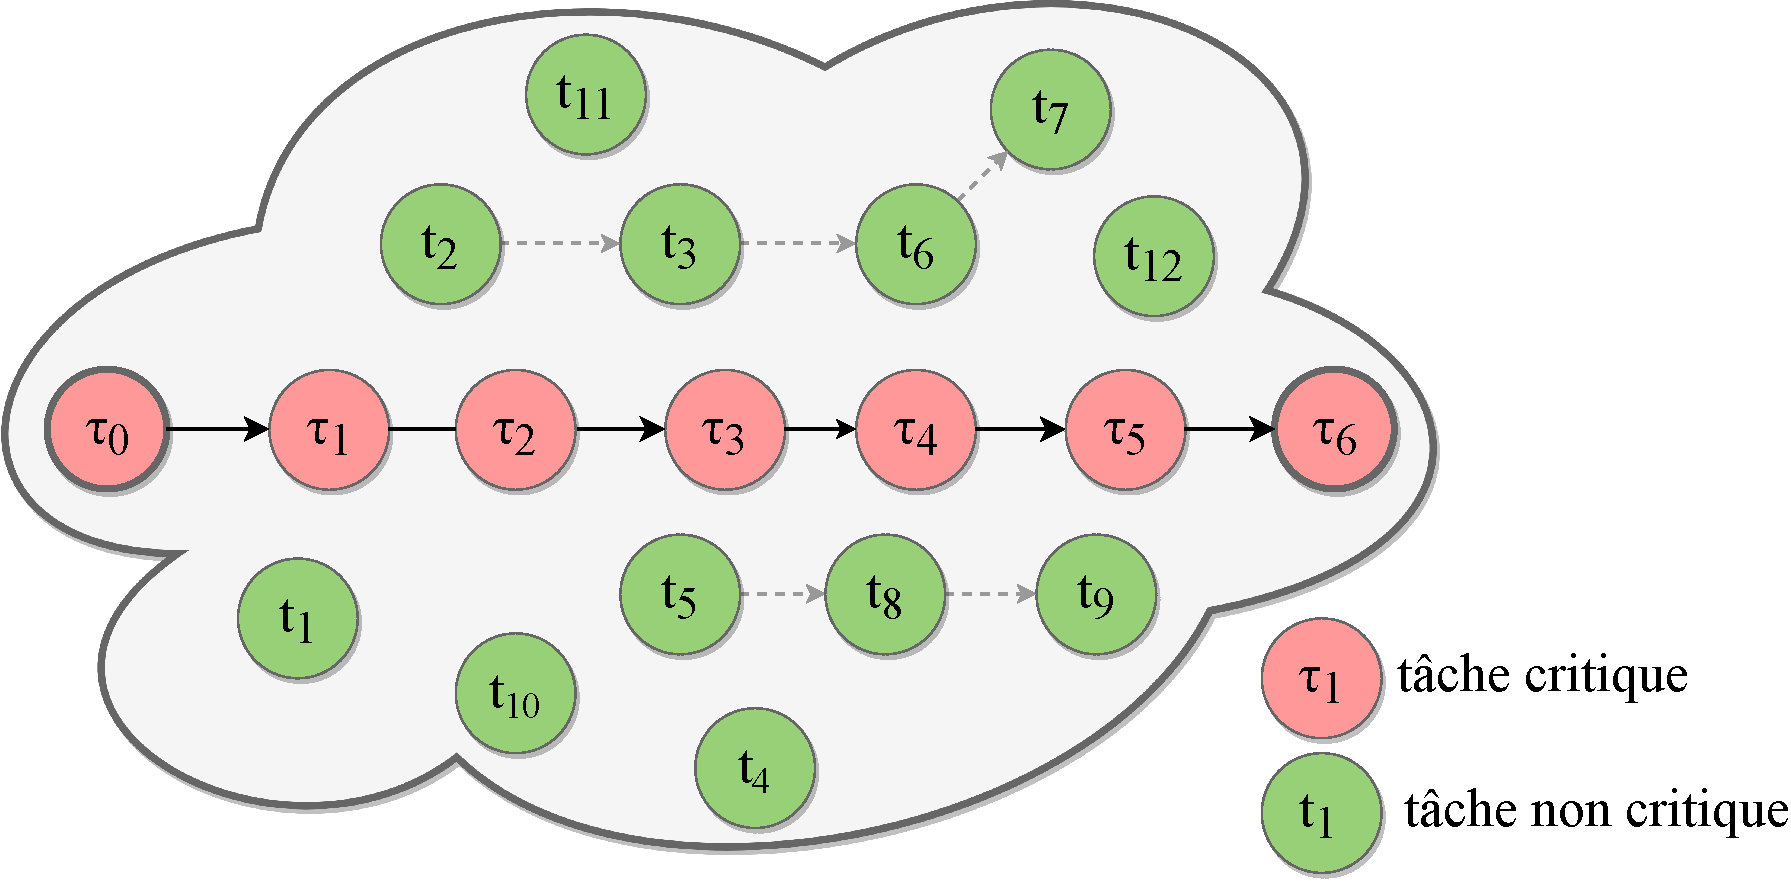
\includegraphics[width=0.8\linewidth]{schemas/Set_de_Taches}
    		\caption{Représentation simplifiée du set de tâches à criticité duale}
    		\label{fig:SetdeTaches}
    	\end{figure}
    	
    	
    	\subsubsection{Modèle de tâches}
		La plupart des hypothèses faites ici se focalisent sur les tâches critiques, tandis que la seule hypothèse forte sur les tâches non critique est la capacité à les stopper (soit un arrêt total, soit une mise en pause) et les relancer en cours d'exécution de façon à pouvoir déclencher un Mode Dégradé où il n'y a plus de tâches non critiques avec les risques d'interférences afférents envers les tâches critiques. Sous les systèmes type Unix, cela correspond typiquement à l'envoi d'un signal SIGSTOP et SIGCONT. Sans cette condition, les Modes de Service mentionnés ci-dessus ne sont pas exploitables pour notre besoin. 
		
		Chaque tâche critique $\tau_i$ est activée et exécutée suivant une période $T_i$. 
		À chaque période, le job $\tau_{i,j}$ correspond à la $j^{ieme}$ exécution de la tâche $\tau_i$. 
		On peut alors noter pour chaque job $\tau_{i,j}$ son moment d'activation $a_{i,j}$, son début d'exécution $s_{i,j}$ et sa terminaison $e_{i,j}$. 
		On considère qu'un job consomme toutes ses données d'entrée (inputs) au début de son exécution, s'exécute et fournit à la fin de son exécution les données de sortie. Les données d'entrée et de sortie des tâches sont stockées en espace mémoire partagé : la transmission des données d'une tâche à l'autre se fait de façon asynchrone.
		Cela nous mène à la question de l'interaction entre les tâches et notamment la façon de représenter la précédence.
		%%%%%%%%%%%%%%%%%%
		%%\alert{Citer différents modèles d'exécution de tâches existants ici ? c.f. ~\cite{friese_estimating_2018}}
    	%%%%%%%%%%%%%%%%%%
    	
    	\subsubsection{Chaînes de tâches}
	    La question de la dépendance entre les tâches est importante pour aborder le problème des contraintes temps-réel avec une vision plus macroscopique. En effet, dans le cadre de l'usage de tâches ayant des contraintes temporelles souples (c.f.~\autoref{sec:SystemesTempsReels} - Systèmes temps-réel), c'est uniquement avec une vision plus globale de l'exécution du système qu'il est possible de tirer au maximum parti des légers dépassements pour éviter dans la globalité d'avoir recours à des politiques d'exécution des tâches plus restrictives, et par conséquent qui sous-exploitent la puissance de calcul disponible.
	    Nous considérons ici la dépendance entre les tâches via les données partagées entre ces dernières selon un modèle type producteurs/consommateurs. Les tâches ont des relations de cause à effet et par conséquent, d'un point de vue strictement fonctionnel on peut décrire le système comme étant une accumulation de fonctionnalités réalisées par l'exécution de tâches successives. Cela permet alors d'introduire la notion de contrainte temporelle fonctionnelle, qui décrivent des contraintes d'exécution de chaînes de tâches bout-en-bout.
	    
	    
	    On représente une dépendance entre tâches sous la forme de chaînes de tâches, suivant le modèle $\tau_{1} \rightarrow \tau_2 \rightarrow \ldots \rightarrow \tau_n$. Dans un tel exemple, $\tau_1$ est la \textbf{tâche d'entrée} de la chaîne, tandis que $\tau_n$ est la \textbf{tâche de sortie} de la chaîne. Notons que ce modèle peut être étendu pour supporter des tâches représentées par un Diagramme Orienté Acyclique (\textit{Directed Acyclic Graph - DAG}) sans difficulté. Nous travaillons dans le cadre de ces travaux avec des chaînes directes, sans divergences ou convergences dans le graphe. De fait, cet ajout de complexité dans le modèle de chaîne de tâches n'apportera pas de différences particulières sur les résultats ni sur la démarche. De fait la différence fondamentale étant sur la façon de monitorer et reconstituer l'état de la chaîne de tâches, ce sont des éléments qui sont modifiables simplement pour prendre en compte un DAG complet. Le reste du principe présenté demeure fondamentalement inchangé.

	    %%%%%%%%%%%%%%%%%%%%%%%%%%
	    %\alert{J'hésite à présenter ça dans "l'autre sens" : présenter un modèle de chaînes de tâches plus complet (avec divergences, convergences, etc.) et au final restreindre le modèle à des chaînes linéaires qu'au niveau du cas d'étude (chapitre 5). Option 2 (actuelle): en perspective de la thèse présenter les implications d'un modèle de chaînes plus complexe}
	    %%%%%%%%%%%%%%%%%%%%%%%%%%
	    \begin{figure}[ht]
	    	\centering
	    	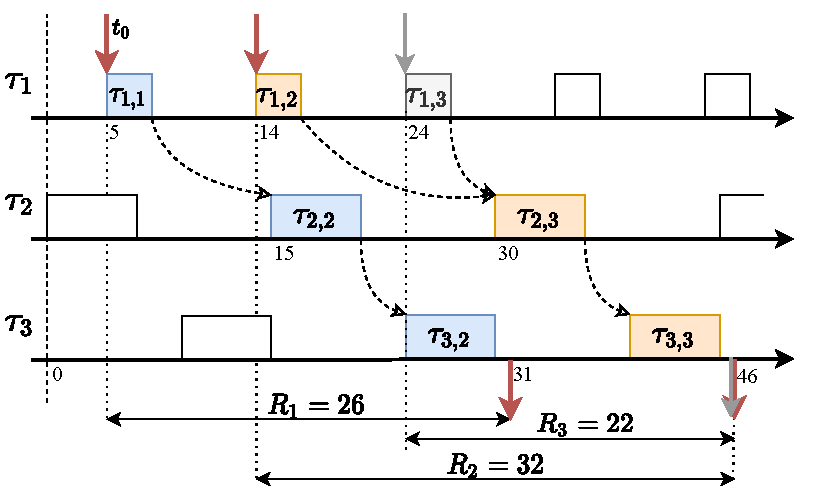
\includegraphics[width=.8\linewidth]{Chronogrammes-TaskChain}
	    	\caption{Exemple d'exécution d'une chaîne de tâches $\tau_1 \rightarrow \tau_2 \rightarrow \tau_3$}
	    	\label{fig:chain_chronogram}
	    \end{figure}
    
	    Dans ce contexte, on définit à l'exécution la précédence entre les tâches par le biais d'un lien type producteur-consommateur. On considère que pour une tâche, les données produites sont disponibles à partir de la terminaison de cette dernière. Chaque tâche dans la chaîne de tâche consommera les données de sortie de tous les jobs de la tâche précédente dans cette chaîne qui n'ont pas encore été consommées au début de son exécution. En regardant l'exemple de la~\autoref{fig:chain_chronogram} avec une chaîne $\tau_1 \rightarrow \tau_2 \rightarrow \tau_3$, à considérer que chaque job est désigné par la notation $ \tau_{i,j} $, $i$ indiquant la tâche et $j$ l'indice d'occurrence d'exécution de cette tâche. On peut voir que le job $ \tau_{2,2} $ consomme les données de $ \tau_{1,1} $, mais pas celles de $ \tau_{1,2} $, étant donné que ce job n'est pas encore terminé à t=15. Aussi, $ \tau_{2,3} $ pourra consommer les données de $ \tau_{1,2} $ et $ \tau_{1,3} $ étant donné qu'elles n'ont pas été consommées précédemment.
	    
	    De façon formelle, on peut définir cette relation entre une tâche $\tau_i$ et son successeur $\tau_{i+1}$. Pour produire la donnée de sortie du job $\tau_{i+1,k}$ de la tâche $\tau_{i+1}$, ce dernier consommes toutes les données d'entrée en attente provenant des jobs $\tau_{i,j}$. Les données en attente étant celles qui n'ont pas été consommé par le job $\tau_{i+1,k-1}$ qui est le job précédent de $\tau_{i+1}$. On peut donc écrire que pour un $\{i,k\}$ donnés, sont consommés les données de tous les jobs $\tau_{i,j}$ tel que $ e_{i,j} \leq s_{i+1, k}$ et $e_{i,j} > s_{i+1, k-1}$. Autrement dit, un job $\tau_{i,j}$ n'a un effet sur $\tau_{i+1,k}$ si et seulement si ce dernier est le premier job de $\tau_{i+1}$ exécuté après la terminaison de $\tau_{i,j}$.
	    
	    \textbf{Remarque de compréhension} : \textit{les indices $j$ et $k$ ci-dessus représentent tous deux la différenciation des jobs pour une tâche donnée ($\tau_1$ pour $j$ et $\tau_2$ pour $k$). Si 2 lettres différentes sont utilisées, c'est uniquement du fait qu'il n'y a pas de relation entre 2 jobs de tâches différentes qui auraient le même indice d'occurrence. D'où la distinction $j$/$k$}.
	    
		Dans ces conditions, on nomme $\tau_{i+1,k}$ le \textbf{successeur} du job $\tau_{i,j}$. On note $succ()$ la fonction qui permet de trouver le successeur d'un job donné tel que~: 
		\begin{multline*}
		\forall i,j \in \mathbb{N}^*, \, \exists \, k \in  \mathbb{N}^*  \textrm{ tel que }  \\
		 succ(\tau_{i,j}) = \tau_{i+1,k} \textup{ avec } e_{i,j} \leq s_{i+1,k} \wedge e_{i,j} > s_{i+1,k-1}
		\end{multline*}
	
	%%% Dépend de l'exécution alors. Si durée < WCET, peut changer les dépendances.
	%   Pourquoi considérer un modèle asynchrone => il existe modèle asynchrone faiblement couplé déterministe.
	%   c.f Semaphore Precedence COnstraint (SPC).
	
		Par extension, la fonction itérative $succ^{p}()$ pour tout $p \geq 0$ permet de trouver le p\up{ème} job successeur d'une tâche donnée de la chaîne de tâches. Et in fine, $succ^{n-1}(\tau_{1,j})$ désigne le job de sortie de la chaîne de tâche désignée par son job d'entrée $\tau_{1,j}$. On notera que pour $p = 0$, on définit $succ^{\,0}(\tau{i,j}) = \tau_{i,j}$, soit la fonction identité.
		
		Pour illustrer cela, on peut reprendre l'exemple de la chaîne représentée en~\autoref{fig:chain_chronogram}. On peut par exemple voir qu'une des exécutions de la chaîne de tâche, débutant par $\tau_{1,1}$, donne : $succ^{2}(\tau_{1,1}) = succ(succ(\tau_{1,1})) = succ(\tau_{2,2}) = \tau_{3,2}$. Mais aussi que le job $ \tau_{2,3} $ doit prendre en compte les valeurs de sorties de 2 jobs de la tâche $ \tau_1 $. Plus précisément, $succ(\tau_{1,2}) = succ(\tau_{1,3}) = \tau_{2,3} $. %On a alors le temps de réponse de la-dite chaîne : $R_1 = e_{3,2} - s_{1,1} = 31 - 5 = 26$ unités de temps.
		En effet, étant donné que les tâches peuvent être définies par des périodes d'activation différentes, cela signifie notamment que si une tâche $\tau_i$ est exécutée plus fréquemment que son successeur $succ(\tau_{i+1})$, alors il est possible  qu'un job $\tau_{i+1,j}$ soit le successeur de plusieurs jobs de la tâche $\tau_{i}$.
		
		Par extension et commodité d'usage, on ajoutera comme notations utiles $succ(a_{i,j}), \quad succ(s_{i,j}), \quad succ(e_{i,j})$ respectivement les temps d'activation, de début d'exécution et de terminaison du successeur du job $\tau_{i,j}$. Et de même par fonction itérative, $succ^k(s_{i,j})$ la date de début du k\up{ième} successeur de la tâche $\tau_{i,j}$~: 
		
		\begin{align*}
%%			\textup{Soit } succ(\tau_{i,j}) = \tau_{i+1,k} \textup{, alors :}	\\
		\textup{Soit } succ(\tau_{i,j}) = \tau_{i+1,k} \textup{, alors }
			succ(a_{i,j}) = a_{i+1,k} 	\\
			succ(s_{i,j}) = s_{i+1,k}	\\
			succ(e_{i,j}) = e_{i+1,k}	\\
		\textup{De même, si } succ^n(\tau_{i,j}) = \tau_{i+n,k} \textup{ alors }
			succ^n(a_{i,j}) = a_{i+n,k}		\\
			succ^n(s_{i,j}) = s_{i+n,k}		\\
			succ^n(e_{i,j}) = e_{i+n,k}
		\end{align*}
	    
  		 Cette façon de considérer les choses permet une plus grande flexibilité de notre modèle pour s'adapter à un cas concret. De cette façon le modèle gère déjà un nombre assez significatif d'implémentations de tâches existantes~:
	\begin{itemize}
		\item   		Des tâches avec une file d'attente en entrée : lorsque la tâche est exécutée elle consomme toutes les données d'entrée en attente -- le cas de base que nous considérons.
		\item   		Des tâches qui ne consomment que la donnée d'entrée la plus récente, les données précédentes étant considérées obsolètes. Dans ce cas-là, c'est équivalent à considérer que toutes les données précédentes sont consommées, mais qu'uniquement la plus récente est prise en compte, celles des jobs plus anciens sont ignorées.
		\item   		Pour les tâches où chaque exécution de la tâche ne prend en compte qu'une seule donnée en file d'attente, notre modèle ne gère pas tous les cas. Cela peut être la donnée la plus ancienne (stratégie FIFO\footnote{FIFO : First-In First-Out, les données sont traitées de la première arrivée à la dernière.}) ou la plus récente (stratégie LIFO\footnote{LIFO : Last-In First-Out, les données sont traitées de la dernière (plus récente) arrivée à la plus ancienne.}). Quoi qu'il en soit, notre capacité à prendre en compte ce type de tâche va être dépendant de leur fréquence d'activation. 
		\begin{enumerate}
			\item 	Si les tâches s'exécutent toutes à la même fréquence, alors il y aura systématiquement une relation 1\string:1 entre producteurs et consommateurs.
			\item 	Si les tâches successeur dans une chaîne donnée s'exécutent systématiquement à une plus grande fréquence que les tâches précédentes, alors nous sommes aussi dans un cas avec jamais plus d'une donnée disponible en file d'attente. En effet, la tâche Consommateur s'exécutant plus rapidement que la Tâche productrice, le ratio Production/Consommation est inférieur à 1.
		
		Ces 2 cas sont donc équivalents au premier type de tâches mentionné pour lequel toutes les données produites sont consommées, mais où la quantité de données en attente est systématiquement inférieure ou égale à 1 en réalité.
			\item 	En revanche si une tâche successeur dans une chaîne s'exécute plus lentement que sa prédécesseure, c'est le cas qui n'est pas géré par ce modèle. En effet, si une seule donnée est consommée par job, et le reste stocké en file d'attente, alors il pourrait y avoir un ratio Production/Consommation supérieur à 1. C'est-à-dire une plus grande quantité de données produites que consommées. Ce cas est relativement improbable (à moins d'une erreur de conception), car cela implique que la quantité de données en file d'attente peut potentiellement diverger. Or la file d'attente ne peut être considérée infinie.
		\end{enumerate}  
	\end{itemize}
	%%% ça semble bof bof en fait tout ça...
	%   c'est vrai en moyenne, mais en l'absence de mécanisme de synchronisation pas forcément...
	
  		De façon succincte, quand on parle de consommer plusieurs jobs de la tâche précédente tel qu'on le présente ici, cela n'implique pas que toutes ces données seront prises en compte. Tout dépend du modèle de fonctionnement interne des tâches. Mais quoi qu'il en soit, cela permet de gérer un grand nombre de comportements classiques.
  		
  		Nous ne considérons pas dans notre modèle d'éventuels délais entre l'instant où une tâche produit sa donnée de sortie et le moment où cette donnée est réellement disponible pour la ou les tâches consommatrices. Il faudrait pour cela ajouter dans notre modèle de précédence une constante de latence correctement estimée selon l'implémentation de la transmission des données entre les tâches. On pourra noter sur ces aspects les travaux de~\cite{friese_estimating_2018} qui ont pu aborder la prise en compte de latences dans différents modèles de chaînes de tâches.


        \paragraph{Temps de réponse bout-en-bout}

    La notion de successeur permet de définir le temps de réponse bout-en-bout $R_j$ de la $ j $-ème instance d'exécution d'une chaîne de tâche. Ainsi $R_j$ désigne le temps écoulé entre l'activation du \textit{job} d'entrée $\tau_{1,j}$ de la chaîne, jusqu'à la terminaison du \textit{job} de sortie $\tau_{n, k} = succ^{n-1}(\tau_{1,j})$.
    On a alors $R_{j} = succ^{\,n-1}(e_{1,j}) - a_{1,j}$ que l'on peut retrouver dans l'exemple du~\autoref{fig:chain_chronogram}. Sur cet exemple, il est possible de reconstituer trois instances d'exécution de la chaîne de tâches avec les trois temps de réponse correspondants : $R_1$, $R_2$, $R_3$. 
    %Parmi ces instances, on remarque que 2 d'entre-elles sont très semblables, avec le même job de terminaison $ \tau{3,3} $.
    
	Intuitivement, l'échéance bout-en-bout représente alors la durée maximale acceptable pour qu'une donnée d'entrée de la chaîne ait un effet du côté de la sortie. Pour une fonctionnalité donnée on comprend bien que cette échéance doit être bornée, et qu'il faut donc des garanties pour que tout se passe bien de bout-en-bout. Lorsque l'on considère l'échéance d'une chaîne de tâches $D_c$, pour éviter toute faute temporelle de non-respect d'échéance, il faut a minima respecter~:  $\max_{j \in \mathbb{N}}\{R_j\} \leq D_c$.
	
	\smallbreak 
	
	L'objectif à présent est de proposer une approche qui permette justement d'exploiter ces contraintes bout-en-bout, de façon à éviter les risques de fautes temporelles au niveau fonctionnel. Cela se traduit par la volonté de prévenir les risques de dépassement d'échéances, non pas au niveau de chaque tâche individuelle, mais plutôt à un niveau d'observation au-dessus qui est en lien direct avec la représentation fonctionnelle.
	
    
\section[Mécanisme d'anticipation]{Mécanisme d'anticipation \\ par Surveillance et Contrôle}
    \subsection{Méthode d'anticipation}
    
 %%% Question Grolleau 
 %   Les tâches sont strictement périodiques ? Basées sur même horloge ?
    Je propose donc un mécanisme basé sur la surveillance à l'exécution de l'avancement d'une chaîne de tâches. 
    Pour ce faire, on introduit les notions d'\textbf{État de Chaîne de Tâches} et de \textbf{Trace d'Exécution de Chaîne de Tâches}. Une chaîne de tâches donnée est associée à un État et plusieurs Traces d'Exécutions. Ces deux éléments évoluant au fil de l'exécution du système, on peut noter $S(t)$ l'État à l'instant t et $ET(j,t)$ la j\up{ème} Trace d'Exécution de la Chaîne de tâches à l'instant t.
    
    On peut alors définir pour une Chaîne de Tâches dont la tâche d'entrée est $\tau_{1}$, et la tâche de sortie $\tau_{n}$ : 
    \begin{definition} \label{def:TraceExecutionChaine}
    	Une \textbf{Trace d'Exécution} $ET(j,t)$ se définit par le début d'exécution d'un job d'entrée $s_{1,j}$ ainsi que tous les temps de fin d'exécution $e_{i,j}$ des \textit{successeurs} itératifs de ce job qui ont été identifiés à l'instant $t$.
    	\begin{equation*}
    		ET(j,t) = \{\: a_{1,j} \:,\: e_{1,j} \:, succ(e_{1,j})\:, \;\dots\; ,\: succ^{n-1}(e_{1,j}) = e_{n,k} \:\}
    	\end{equation*}    	
    	Une Trace d'Exécution $ET(j,t)$ est dite \emph{active} si son job de départ $\tau_{1,j}$ a déjà été activé à l'instant t, et que son successeur itératif correspondant à la tâche de sortie de la chaîne $\tau_{n,k}$ n'a pas encore été terminé. Autrement, elle est \textit{inactive}. En d'autres termes :
    	\begin{equation*}
    		ET(j,t)  \quad \textrm{est active ssi}\quad  a_{1,j} \leq t \quad \textrm{et} \quad e_{n,k} > t
    	\end{equation*}
    \end{definition}
    
    %Our anticipation mechanism is based on the run-time monitoring of the task chain progress. 
    %To that end, we introduce the notions of \textbf{Task Chain State} and \textbf{Task Chain Execution Trace} (TCET). 
    %A TCET contains an entry task job and all the iterative successors of that job. 
    %At a time $t$ a TCET can be \emph{active}, if its entry task job has been activated and if its exit task job has not yet ended, or \emph{inactive} otherwise. 
    
    Il est possible de définir à partir des Traces d'exécution, actives ou inactives à un instant $t$, l'État de la Chaîne de tâches :
    
    \begin{definition}\label{def:EtatChaine}
    	L'\textbf{État d'une Chaîne de Tâches} $S(t)$ définit à un instant $t$ l'état d'avancement de l'exécution de la chaîne de tâches qui est toujours en cours et qui a été activée la plus anciennement. Autrement dit, $\pmb{S(t) =\langle t_0, \tau_p\rangle}$ basé sur la Trace d'Exécution la plus ancienne active $ ET(j,t) $ tel que~:
    	\begin{equation*} 
    		\left|
			\begin{array}{ll}
				\displaystyle	t_0 &= \displaystyle\min_{j \in \mathbb{N}^*} \left\{ a_{1,j} \mid
			    	  					a_{1,j} \leq t \wedge succ^{n-1}(e_{1,j}) > t \right\}		\\
			    \displaystyle	\tau_p = succ^{\,p}(\tau_{1,j}) &= \displaystyle\min_{l\,\in\,[\![0;n-2]\!] } \left\{ succ^{\,l+1}(\tau_{1,j}) \mid succ^{\,l}(e_{1,j}) \leq t \right\}
			\end{array}
    	  	\right.
    	\end{equation*}
    Avec $t_0$ la plus ancienne activation parmi les $ET(j,t)$ et $\tau_p$ la prochaine tâche de cette trace d'exécution qui n'a pas encore été terminée.
    \end{definition}

    De cette façon, l'État d'une chaîne de tâches indique quelles sont les tâches restantes à exécuter dans la chaîne à un instant donné et son temps de réponse partiel actuel que l'on notera $RT(t) = t - t_0$. L'état de la chaîne se focalise sur la chaîne active la plus ancienne, donc la plus longue ce qui implique que c'est la plus à même de dépasser l'échéance.
    
    Pour finir, au regard de l'État d'une chaîne de tâches, on peut s'intéresser au temps restant jusqu'à la complétion de cette chaîne. Il est possible d'estimer le temps qu'il faudra pour aller jusqu'à exécuter la tâche de sortie de la chaîne qui fait partie de la Trace d'Exécution active observée, c'est-à-dire $succ^{\,n-1}(\tau_{1,j}) = \tau_{n,j}$. Et si, de plus, cette estimation est faite dans les hypothèses d'estimation de Temps d'Exécution Pire Cas, on obtient alors une estimation de \textbf{\emph}{Pire Temps de Réponse restant} $rWCRT(t)$ à l'instant $t$ pour terminer l'exécution de la trace d'exécution active la plus longue.
    
    Alors, en combinant l'État à un instant $t$ avec une estimation du Temps de Réponse Pire Cas restant, on peut donc estimer une borne haute garantie de temps de réponse de la chaîne de tâche. C'est là que l'on peut faire entrer en jeu un mécanisme d'anticipation. 
    On dispose pour une chaîne de tâches donnée de son temps de réponse partiel actuel ainsi qu'une estimation de temps de réponse restant en pire cas. Il est alors possible de déterminer s'il y a un risque de défaillance par dépassement de l'échéance bout-en-bout $D_c$.
    \begin{theorem}[Risque de dépassement d'échéance]
    	Si à un instant donné $t$, l'inéquation suivante est respectée, alors il y a risque de dépassement d'échéance.
    	\begin{equation*} 
    		RT(t) + rWCRT(t) > D_c
    	\end{equation*}
    \end{theorem}

	Pour illustrer cette logique, on peut voir sur le chronogramme~\ref{fig:chronogram_rWCRT_example} à nouveau un exemple avec une chaîne de tâches $\tau_1 \rightarrow \tau_2 \rightarrow \tau_3$. À l'instant $t=18$ d'indiqué il y a deux Traces d'Exécution actives (chaînes reliées par une flèche de succession). On a de ce constat l'État de la chaîne $S(t) = \langle \tau_0, \tau_2\rangle = \langle 4, \tau_{2} \rangle $.
	On en déduit $ RT(18) = t - t_0 = 18-4 = 14 $. Si l'on ajoute à cela une estimation du Temps de Réponse Pire Cas restant $rWCRT(18)$, qui est le temps estimé pour que $\rightarrow \tau_2 \rightarrow \tau_3$ soit exécuté selon les contraintes de précédence, alors on a l'estimation du Pire Temps de Réponse : $ RT(18) + rWCRT(18) = 33$ que l'on peut comparer à la date d'échéance $ D_c = 30 $. Dans cet exemple, il existe donc un risque de dépassement de l'échéance.
	Il est à noter aussi que dans cet exemple l'instant $t$ a été pris en plein pendant l'exécution de la tâche $ \tau_2 $. Ce qui est pris en considération comme si cette dernière n'était pas exécutée. Si l'on ne prend pas non plus en compte son exécution partielle, c'est parce que d'un point de vue externe à cette tâche, sans l'instrumentaliser il n'est pas possible de le savoir. Et de fait, l'une de nos contraintes est d'être le moins intrusif possible sur le code, notamment pour les cas où certains logiciels ne sont pas modifiables (black-box ou legacy). 
	
    \begin{figure}[ht]
		\centering 
		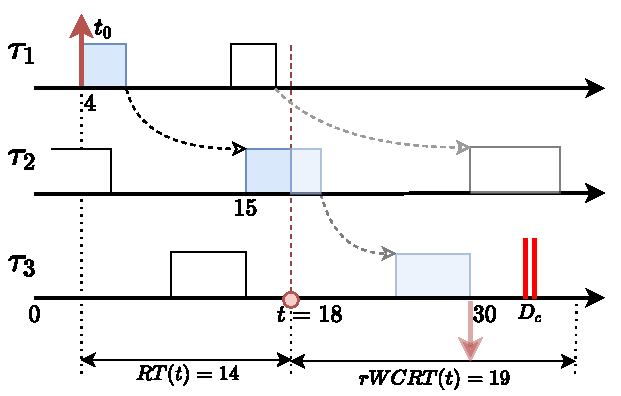
\includegraphics[width=0.7\linewidth]{Chronogrammes-rWCRT-example}
		\caption{Chronogramme de calcul du risque de dépassement à un instant t}
		\label{fig:chronogram_rWCRT_example}
	\end{figure}

	À présent, il faut nous souvenir de notre objectif dans tout cela. Pourquoi vouloir anticiper une défaillance de la sorte ? L'objectif est d'anticiper un risque de dépassement d'échéance à l'échelle d'une chaîne de tâches, de façon à pouvoir passer d'un Mode d'ordonnancement Nominal vers un mode Dégradé dans lequel on va prévenir la défaillance. Cette dernière a pour origine première les interférences matérielles qui augmentent les temps d'exécution des tâches. Aussi pour éviter davantage ce glissement temporel et donc conserver la garantie de terminaison de la chaîne de tâches avant l'échéance, on remonte à la source en prévenant temporairement tout risque d'interférences. Et cela est obtenu via un mode dégradé dans lequel la méthode consiste à stopper temporairement les tâches non critiques, cause des interférences.
	Il nous faut décrire à présent la méthode de passage en mode dégradé.
	

    
    \subsection{Passage en Mode Dégradé}
    
        \paragraph{Estimation de Temps d'Exécution Pire Cas restant}
    Bien évidemment, l'estimation du Temps de Réponse Pire Cas restant est un élément clé de l'approche. Tout l'intérêt de cette méthode réside dans la capacité à passer dans un mode dégradé. En conséquence, ce que nous nous devons de garantir, c'est le non-dépassement d'échéance sachant qu'il est possible à tout moment de prendre la décision du passage en mode dégradé, dans lequel les tâches critiques n'étant plus sujettes à interférences externes, auront un Temps d'Exécution Pire Cas bien plus faible qu'en mode Nominal. 
    Cela implique directement que si le $rWCRT(t)$ que nous considérons est dans le contexte Dégradé, alors la détection d'un éventuel risque se fait de façon beaucoup plus permissive que si l'on considère directement les risques en mode Nominal. 
    Étant donné que le mode dégradé correspond à un arrêt des tâches non critiques, on peut considérer que dans ce mode la chaîne de tâches est en isolation. De ce fait, la seule chose qui va modifier l'estimation du $rWCRT(t)$ va être l'État de la chaîne de tâches à l'instant t, $S(t)$. Or, étant donné que $S_c = \langle t_0, \tau_i\rangle$, alors on remarque qu'il n'y a que la valeur de $\tau_i$ -- c'est-à-dire la prochaine tâche de la chaîne qui doit être exécutée -- qui va influer sur la valeur estimée du pire temps de réponse restant. Ainsi, $rWCRT(t)$ peut être simplifié en une fonction discrète qui évolue avec $S(t)$. Par conséquent, on notera pour la suite de notre raisonnement $rWCRT(t) = rWCRT(\tau_i)$. 
    
    Ceci étant posé, il existe plusieurs méthodes à l'estimation de $rWCRT(\tau_i)$. 
    De façon théorique, il est possible d'exploiter les méthodes déjà existantes d'estimation de temps d'exécution pire cas, auxquelles il faut ajouter la prise en compte des temps d'activation des tâches. Ce type d'approche devient hautement dépendante du système étudié, que ce soit l'architecture matérielle, mais surtout la politique d'ordonnancement des tâches, le type de tâches (périodique, sporadique, interruption)... De façon générale, la complexité des approches théoriques n'est pas négligeable et, il faut l'admettre, hors de notre cadre d'expertise. C'est d'autant plus vrai dans un cas d'application sur processeur multicœur pour lequel il est facile de tomber dans des estimations trop pessimistes. Pour cette raison, nous avons décidé dans notre proposition d'avoir une approche plus expérimentale.
    
    %To help with the estimation of $rWCRT$, we assume that the HI-criticality task chain execute on a single core. To avoid interference between the MCA and the task chain we prevent the MCA to use the same core. Lo-criticality tasks can execute on any core as depicted on \autoref{fig:SoftwareArchitecture}. 

    Un avantage dont nous bénéficions ici, c'est que l'hypothèse de se ramener à un cas en isolation dans le mode dégradé limite grandement les risques de variations sur les temps d'exécutions des tâches critiques. C'est ce qui permet une plus grande certitude sur les estimations expérimentales, qui ne nécessitent alors plus de couvrir toute une combinatoire incluant les tâches non critiques. L'estimation est donc faite expérimentalement en exécutant le système avec un passage forcé en mode dégradé dans lequel on peut alors mesurer sans les tâches non-critiques les Temps de Réponse Pire Cas restants $rWCRT(\tau_i)$. On notera que pour une chaîne de N tâches, il y a N-1 $rWCRT$ à estimer. Plus de détails sur le protocole adopté pour l'estimation seront abordés en~\autoref{chap:4_ProtocolExpe}.

    La transition en elle-même vers le mode dégradé est une phase importante du fait qu'elle implique des délais supplémentaires qui devront être pris en compte dans l'anticipation. De cette façon, à considérer que l'on recalcule périodiquement le risque de dépassement d'échéance, il est possible de définir l'instant où l'on sait que l'attente d'une période supplémentaire va faire que même en mode dégradé, il ne sera plus possible de garantir le respect de l'échéance bout-en-bout. Par conséquent, il devient alors clair que cet instant-là devient le dernier moment auquel il faut nécessairement passer en mode dégradé pour justement conserver cette garantie.

%The MCA role is first to monitor the state of a HI-criticality task chain to detect potential deadline miss. If such a potential fault is anticipated, then the MCA switches the system to HI-criticality mode, pausing all non essential workload (LO-criticality tasks), to prevent further interference on the HI-criticality tasks and allow a safe termination. To be efficient, the switch  must be triggered only when necessary (as a “mode switch procrastination”, as called in~\cite{hu_ffob_2019}). That is why we also focus on end-to-end deadline, rather than individual task deadlines, in order to avoid false-positive switching, meaning switching to HI-criticality mode although there is slack in the task chain. Indeed, with an end-to-end perspective, we can use the slack given by a task finishing early to compensate the lateness of an other task in the chain.

	\paragraph{Transition de Mode}
    Ce changement de mode se fait en 3 étapes. Il faut en premier lieu bien entendu la détection du point de bascule auquel le risque de défaillance est détecté, c'est l'étape de décision. Une fois la décision prise, la seconde étape est d'activer le mécanisme de passage en mode dégradé. Dans notre cas, il s'agit d'envoyer un signal aux tâches non critiques de façon à mettre en pause leur exécution, c'est l'étape de contrôle. Enfin, le système de surveillance doit continuer d'observer l'État de la chaîne de tâches de façon à relancer les tâches non critiques une fois le risque passé. Il s'agit de l'étape de recouvrement.
    
    Ces trois étapes font ressortir un élément important pour l'anticipation qui n'a pas été pris en compte pour le moment, et il s'agit de la durée entre l'étape de décision et la fin de l'étape d'exécution. En effet, le temps pour que toutes les tâches non critiques soient mises en pause est non nul, et ce délai doit être pris en compte dans l'estimation de Temps d'Exécution Pire Cas restant. %dans l'optique où le pire cas en question est considéré dans le mode dégradé.
    
	En conclusion, en considérant les grandeurs suivantes : 
	\begin{itemize}
		\item 	$ W_{MAX} $ La durée maximum garantie entre 2 points de surveillance de l'Etat de la chaîne de tâche
		\item 	$ t_{SW} $ Le délai maximum nécessaire à la transition du mode nominal au mode dégradé
		\item 	$ rWCRT(\tau_i) $ pour chaque $\tau_i$ de la chaîne de tâche, les Temps de Réponses Pire Cas restant en mode dégradé
	\end{itemize}
	Il est alors possible de calculer la somme du temps de réponse partiel actuel avec ces trois métriques. Tant que cette somme reste inférieure à l'échéance bout-en-bout, alors on peut conserver le système en mode nominal. En revanche, à partir du moment où cela dépasse l'échéance, alors c'est le moment où il n'est plus sûr de rester en mode nominal, et il faut donc déclencher le mode dégradé pour garantir le respect de l'échéance. Cela correspond en conséquence à surveiller que l'inéquation suivante reste vraie pour savoir l'instant critique auquel il faut passer en mode dégradé~:
	
	\begin{theorem}[Condition de passage en mode dégradé]
		Tant que l'inéquation~\ref{eq:safe_cond} est vraie, alors il est toujours possible de garantir le respect de l'échéance bout-en-bout de la chaîne de tâches critiques pour la durée $W_{max}$ sans passer en mode dégradé.
		\begin{equation} \label{eq:safe_cond}
			RT(t) + rWCRT(\tau_i) + W_{max} + t_{SW} \leq D_c
		\end{equation} 
	\end{theorem}

	Cette équation est notamment adaptée des travaux de~\cite{kritikakou_run-time_2014}. Chaque point de surveillance de l'État de la chaîne de tâches est considéré comme étant temporellement sûr (au sens où il n'y a pas de risque de faute temporelle due au dépassement d'échéance) tant que cette inégalité est respectée.
    
    \begin{proof}
		En présumant que (\ref{eq:safe_cond}) est respectée, on peut montrer qu'il est sûr d'attendre le prochain point de surveillance pour décider de changer de mode. \nline
		À l'instant de surveillance $t$, soit $t_{next}$ le prochain instant de surveillance.\nline
		Par définition, $t_{next} \leq t + W_{max}$. Alors $RT(t_{next}) \leq RT(t) + W_{max}$. 
		Par conséquent, \smallbreak
		$RT(t_{next}) + rWCRT(\tau_i) + t_{SW} \leq RT(t) + rWCRT(\tau_i) + W_{max} + t_{SW}$. \nline
		Aussi, $rWCRT()$ ne peut que décroître avec le temps qui s'écoule. Par conséquent, %\smallbreak
		\[ rWCRT(t_{next}) \leq rWCRT(\tau_i)	\]
		et 
		\[ RT(t_{next}) + rWCRT(t_{next}) + t_{SW} \leq RT(t) + rWCRT(\tau_i) + W_{max} + t_{SW} \] 
		Étant donné que l'inégalité (\ref{eq:safe_cond}) est respecté, on a $RT(t_{next}) + rWCRT(t_{next}) + t_{SW} \leq D_c$.
		De ce fait, il sera sûr de passer en mode dégradé au prochain point de surveillance.  
    \end{proof}
    
%    \begin{figure}[ht]
%    	\centering
%    	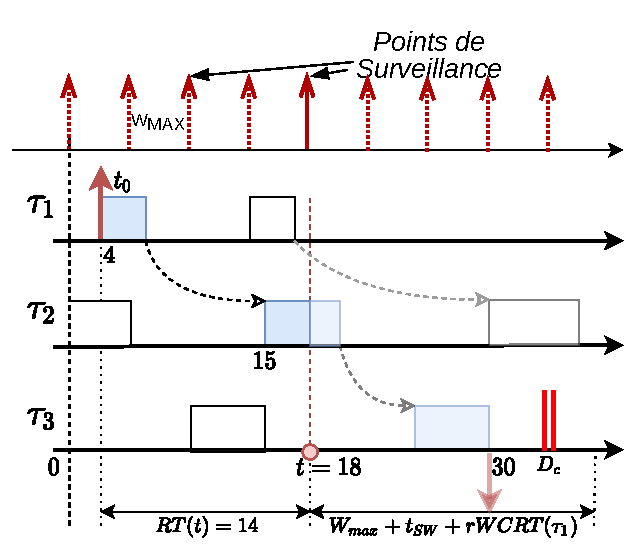
\includegraphics[width=0.92\linewidth]{schemas/chronogram_rWCRT_complet}
%    	\caption{Anticipation de défaillance par changement de mode}
%    	\label{fig:rwcrtchronogram}
%    \end{figure}
	\begin{figure}[ht]
		\centering
		\begin{subfigure}{0.7\textwidth} \centering
			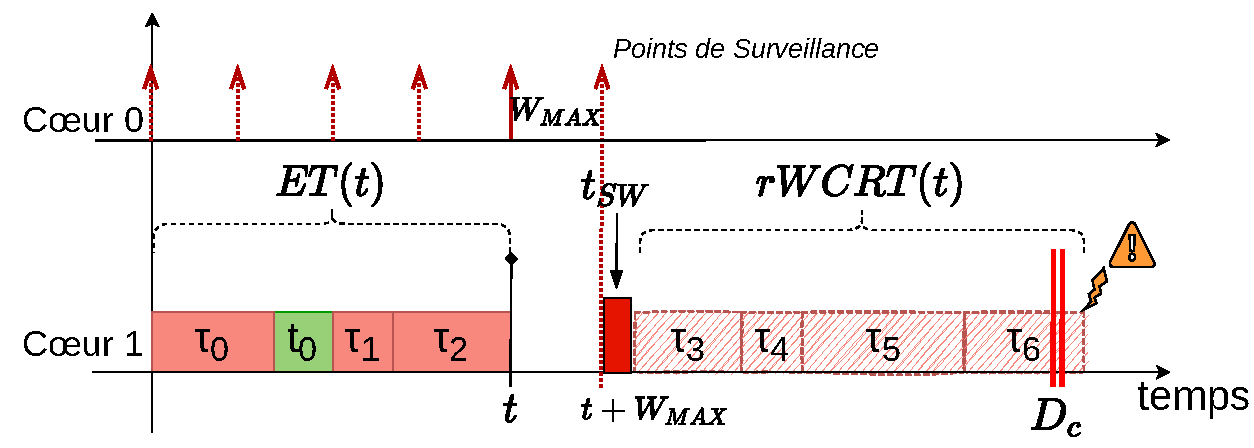
\includegraphics[width=\linewidth]{Chronogrammes-Anticipation_Defaillance}
			\caption[Anticipation - risque de défaillance]{Anticipation - calcul du risque de défaillance}
			\label{sufig:chrono_risque_defaillance}
		\end{subfigure}
		\begin{subfigure}{0.7\textwidth} \centering
			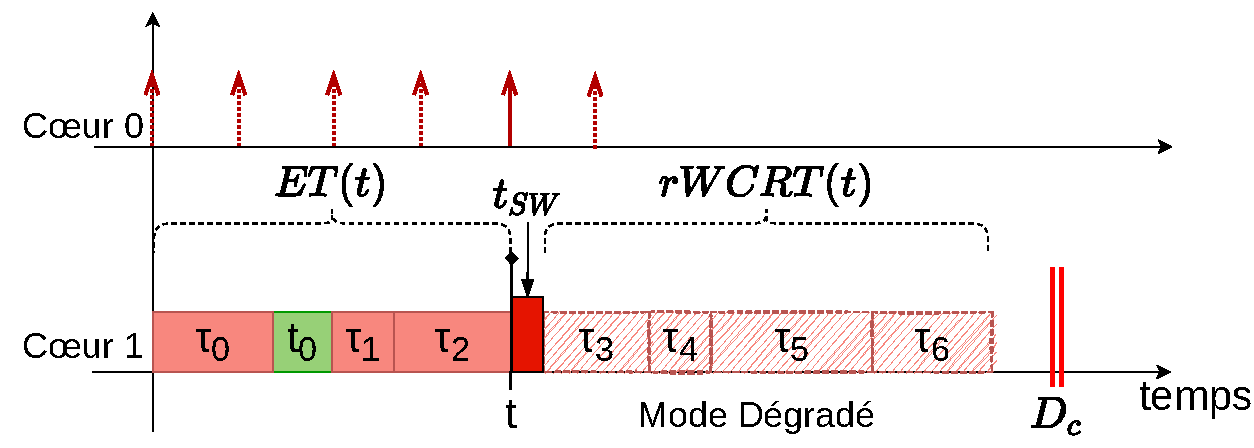
\includegraphics[width=\linewidth]{Chronogrammes-Anticipation_Corrigee}
			\caption[Anticipation - passage en mode dégradé]{Anticipation - déclenchement du passage en mode dégradé}
			\label{sufig:chrono_risque_ModeDegrade}
		\end{subfigure}
		\caption{Chronogrammes de fonctionnement du mécanisme d'anticipation}
		\label{fig:rwcrtchronogram}
	\end{figure}

    En conclusion, grâce au calcul d'anticipation de risque de dépassement d'échéance, il nous est possible d'identifier l'instant $t$ auquel il est nécessaire de passer en Mode Dégradé. La démarche que suit notre mécanisme d'anticipation est illustrée en~\autoref{fig:rwcrtchronogram} avec l'hypothèse d'une chaîne de tâche~:    \[ \tau_{0} \rightarrow \tau_{1} \rightarrow \tau_{2} \rightarrow \tau_{3} \rightarrow \tau_{4} \rightarrow \tau_{5} \rightarrow \tau_{6} \] 
     
     À chaque point de Surveillance, le mécanisme anticipe le risque en calculant l'inégalité \ref{eq:safe_cond} comme reconstitué en~\autoref{sufig:chrono_risque_defaillance}. Si l'inégalité n'est plus respectée et donc que le risque est manifeste comme sur le chronogramme, alors le passage en mode dégradé est effectué, de façon à ce que ce soit le scénario représenté en~\autoref{sufig:chrono_risque_ModeDegrade} qui se réalise, et donc éviter le dépassement d'échéance potentiel. On notera la présence de la tâche non critique $t_0$ qui s'exécute sur le même cœur mais n'influe pas sur le calcul d'anticipation qui est fait.
	%La méthode de réglage de la période de surveillance sera discuté dans le~\autoref{chap:4_ProtocolExpe}.
	
	\section{Architecture Logicielle}
	
	Maintenant que nous avons présenté toute la logique derrière le mécanisme de surveillance et de contrôle, nous allons présenter plus en détail l'architecture logicielle nécessaire à son implémentation.
	
	Pour résumer, nous sommes dans le cas d'un système à criticité mixte implémenté sur un calculateur multicœur, dans lequel nous avons distingué une chaîne de tâches critiques des autres tâches considérées non-critiques. Nous souhaitons ajouter un Agent de Surveillance et de Contrôle pour assurer la fonctionnalité de mitigation des fautes temporelles sur la chaîne de tâches critique. Ce dernier se destine à être exécuté en couche bas niveau, au même niveau que la politique d'ordonnancement du système. Dans le cadre de la suite de nos expérimentations, pour simplifier l'implémentation, nous avons considéré l'isolation de l'Agent de Surveillance et Contrôle sur un cœur du processeur. L'ensemble de ces éléments se résume en~\autoref{fig:SoftwareArchitecture}.

	\begin{figure}[ht]
        \centering
        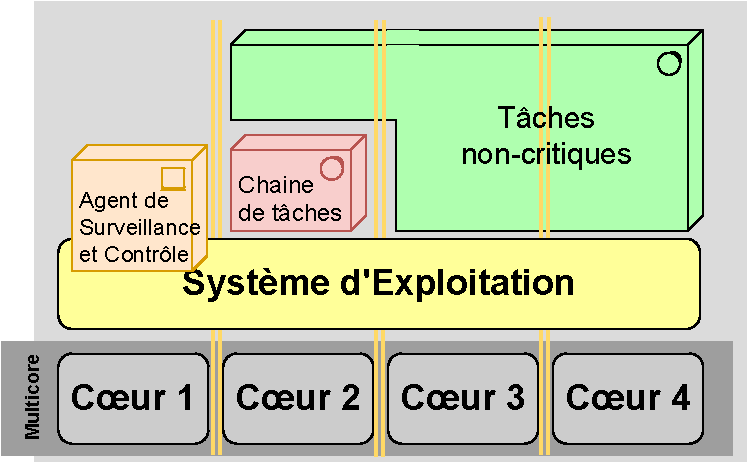
\includegraphics[width=.6\linewidth]{ArchitectureLogicielle.pdf}
        \caption{Architecture Conceptuelle du mécanisme de Surveillance et Contrôle} \label{fig:SoftwareArchitecture}
	\end{figure}

	L'Agent de Surveillance et Contrôle peut se décomposer en deux éléments distincts. D'un part un \emph{Task Wrapper Components} (TWC) et de l'autre le \emph{Core Control Component} (CCC). Le TWC se destine à récupérer toutes les informations nécessaires à la surveillance et la mise à jour de l'État de la Chaîne de tâches par le biais d'une encapsulation des tâches , tandis que le CCC doit prendre en compte ces informations, de façon à réaliser la prise de décision du passage en mode dégradé au regard de l'inéquation~\ref{eq:safe_cond}. Les interactions entre les différents composants logiciels sont représentées sur la~\autoref{fig:architecture}.
	
	
        \begin{figure}[ht!]
            \centering
            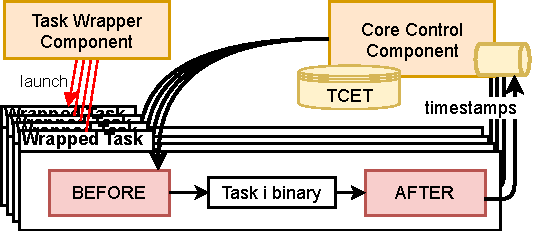
\includegraphics[width=0.7\linewidth]{ArchitectureFramework.pdf}
            \caption{Architecture Logicielle de l'Agent de Surveillance et Contrôle}
            \label{fig:architecture}
        \end{figure}
        
        
        \subsection{Task Wrapper Component (TWC)} 
        
        L'objectif du Task Wrapper Component est de gérer l'aspect Surveillance du mécanisme. Il englobe l'instrumentation du logiciel de façon non intrusive pour obtenir les informations nécessaires à la Surveillance. C'est une différence assez importante avec bon nombre de travaux qui se basent sur la surveillance de l'exécution de tâches. Souvent ces dernières reposent sur une instrumentation logicielle au niveau du code des tâches. Cela offre un suivi plus fin, mais avec un coût de développement logiciel supplémentaire pour chaque tâche. De plus c'est par définition incompatible avec du logiciel fourni en boite noire.
        
        Le mécanisme de Surveillance et Contrôle nécessite \begin{enumerate*}[label=\bfseries\alph*)]
        	\item une connaissance des dates d'activation et de terminaison des jobs, ainsi que 
        	\item la connaissance de la structure de la chaîne de tâche
        \end{enumerate*}. Concernant le premier point, il faut donc ajouter des blocs de code exécutés directement avant le début d'exécution des tâches ainsi que juste avant leur terminaison. En récupérant les \textit{timestamps}\footnote{timestamp~: en informatique, le temps se mesure par un compteur, une variable qui s'incrémente proportionnellement à la fréquence de fonctionnement du processeur. Un timestamp correspond à un horodatage sur ce compteur} d'exécution de ces blocs de code, il est ainsi possible de connaître précisément les dates de début $s_{i,j}$ et de fin $e_{i,j}$ de chaque job. Ils ont vocation à être envoyés au Core Control Component pour mettre à jour l'État de la chaîne de tâches ainsi que le suivi des Traces d'Exécution actives.
        
        Par ailleurs, une telle instrumentalisation permet d'ajouter une couche de sécurité supplémentaire. En effet, le changement de mode se fait initialement par envoi d'un signal pour stopper les tâches non critiques. Ceci étant dit, pour une meilleure réactivité et ajouter de la redondance dans l'arrêt des tâches, il est aussi possible d'utiliser le bloc logiciel exécuté avant l'exécution des tâches non critiques pour vérifier si la tâche en question a effectivement l'autorisation de s'exécuter ou bien si on est en mode dégradé, doit être stoppée. 
        
        En somme, le Task Wrapper Component doit encapsuler les tâches pour ajouter deux wrappers : un \textbf{Before} et un \textbf{After} qui vont avoir deux rôles : 
        \begin{itemize}
        	\item envoyer au Core Control Component les timestamps d'exécution associés à chaque job de tâche critique (dates de début et de fin),
        	\item ajouter de la redondance pour prévenir l'exécution des tâches non-critiques en mode dégradé et potentiellement accélérer le changement de mode.
        \end{itemize}
		On remarquera qu'il n'est pas utile d'exécuter un wrapper After à la suite des tâches non critiques étant donné que nous ne monitorons pas leur exécution dans le cadre du mécanisme.

        \subsection{Core Control Component (CCC)}
        
        Le Core Control Component gère donc l'aspect "Contrôle" du mécanisme. Il doit être exécuté périodiquement, tous les $T_{CCC}$ unités de temps. À chaque exécution, son rôle est de récupérer toutes les données de timestamps du TWC. En ayant connaissance de la structure de chaîne de tâches qui est exécutée, il peut alors reconstruire les Traces d'Exécution telles que définies précédemment (Définition~\ref{def:TraceExecutionChaine}).
        
        À partir des Traces actives, l'État de la chaîne de tâches $S(t)$ est alors mis à jour. Il s'agit de calculer successivement : 
        \begin{itemize}
        	\item $RT(t)$, la durée à partir de la date de départ de la tâche d'entrée,
        	\item $rWCRT(\tau_i)$, le Temps de Réponse Pire Cas restant à prendre en compte selon l'état de la trace d'exécution active.
        \end{itemize} 
	    En y ajoutant les constantes $W_{MAX}$ et $t_{SW}$, l'inégalité~\ref{eq:safe_cond} est re-calculée.
        Dans le cas où elle est toujours respectée, rien ne se produit et le CCC peut attendre la prochaine période de vérification. Dans le cas où elle devient fausse, alors la procédure de changement de mode est enclenchée. %D'une part le TWC reçoit l'information de ce changement en mode dégradé, et d'autre part le signal est envoyé aux tâches non critiques pour être mises en pause.

        Il pouvait y avoir deux choix possibles d'activation du Core Control Component. Soit en le déclenchant de façon évènementielle, à chaque fois que la TWC reçoit une nouvelle donnée de timestamp, soit en le déclenchant de façon périodique indépendamment de l'exécution des tâches. Notre choix s'est porté sur la seconde option pour une raison fondamentale. En effet, bien qu'un déclenchement asynchrone soit plus simple à implémenter d'un point de vue technique, on perd la maîtrise de l'utilisation processeur de notre Agent de Surveillance et Contrôle, ce qui peut être dommageable pour la maîtrise de l'ordonnancement du système. De plus, dans le cas où une défaillance sur la réception des timestamps surviendrait, le CCC pourrait se retrouver dans une attente indéfinie de données, ne mettant alors pas à jour l'État de la chaîne de tâches... et laissant donc passer les risques de faute temporelle. Par conséquent, avec un déclenchement périodique, on obtient une décorrélation du reste du système. De ce fait, quoi qu'il arrive il sera possible à intervalle fixe de déterminer s'il y a un risque. En effet, même en l'absence de nouveaux messages la valeur de $RT(t)$ continue d'augmenter.
        
        
		\subsection{Définition des constantes de Contrôle}
        Il est important de fixer correctement les paramètres constants du CCC, qui sont $t_{SW}$ et $W_{MAX}$.
        Si ces paramètres sont sous estimés, typiquement dans le cas où le temps de passage en mode dégradé est plus long, alors l'inégalité~\ref{eq:safe_cond} pourra devenir tout bonnement fausse. 
        Concernant la durée maximale entre 2 mises à jour de l'État de la chaîne de tâches $W_{MAX}$, pour une Surveillance périodique faite par une tâche avec le plus haut niveau de priorité, cela correspondra à la durée de la période fixée $T_{CCC}$. Là encore on réalise qu'avec une activation sporadique à l'arrivée des messages, cette durée aurait été plus complexe à fixer. 
        
        Cependant, cela repose sur le choix sur la fréquence d'exécution du CCC. Ce choix peut avoir plusieurs conséquences et va donc être sujet à de potentiels compromis. D'une part, un $T_{CCC}$ trop petit signifie une plus forte utilisation des ressources de calcul, ce qui va directement à l'encontre de notre objectif d'optimiser la puissance de calcul. C'est d'ailleurs une problématique courante des mécanismes de Surveillance, d'avoir un impact négatif sur l'usage des ressources du processeur et s'avérer contre-productif.
        
        À l'inverse, plus la période va être longue, plus le mécanisme d'anticipation sera sensible et anticipera des risques de plus en plus improbables. De fait, plus la prochaine date de vérification de l'État de la chaîne est éloignée dans le temps, plus le moindre glissement de temps d'exécution des tâches critiques va laisser penser à un risque de dépassement d'échéance. Cela fait alors augmenter le taux de faux positifs, c'est-à-dire le taux de déclenchements du passage en mode dégradé qui n'étaient pas nécessaires. Par ailleurs, il faut que le Core Control Component puisse soutenir le débit d'arrivée de données d'exécution des tâches critiques, car il n'est pas possible de maintenir en liste d'attente une quantité infinie de messages.
        
        En conclusion, la valeur de $T_{CCC}$ doit être choisie au regard d'une estimation du débit d'exécution des jobs, donc dépendant du nombre de tâches et de leur période d'exécution. 
        
		Une fois qu'un passage en mode dégradé a été effectué, le CCC doit veiller au recouvrement du système pour retourner en mode nominal en temps voulu. Les passages en mode dégradé se veulent les plus intermittents possibles étant donné qu'ils sont le fruit d'une anticipation pour éviter un potentiel dépassement d'échéance. L'objectif est donc de relancer au plus tôt les tâches non critiques. La stratégie choisie est de repasser en mode nominal à la terminaison de la chaîne de tâches qui a provoqué le passage en mode dégradé. Dans ce stade, il n'y a plus aucun risque présent de dépassement et la reprise de contexte des tâches mises en pause peut se faire normalement, sur leur prochaine période d'activation. 
%		\alert{Manque la stratégie de recouvrement !!}
		
        \cmnt{
            One should note that what makes such approach possible is the evolution of the $rWCRT$ at run-time and as the $S(t)$ evolves. It would not be possible to apply such approach when it comes to monitor \& control individual tasks to guarantee their individual deadlines. For individual deadlines, our method would fit only if we are able to monitor tasks timing state ``inside" the tasks execution, i.e. instrumenting the tasks source code to add internal checkpoints. Such approach on individual tasks would discard by definition the use of black box software assumption for instance, and otherwise would need much higher refresh rate frequencies in order to follow individual tasks execution timing state. Such solution is presented for individual tasks in~\cite{kritikakou_dynascore_2017}.
            }
            
\section{Application industrielle}
    \subsection{Spécification fonctionnelle}
    	Notre proposition d'Agent de Surveillance et Contrôle se veut assez générique et permissive en termes de contraintes d'implémentation de façon à pouvoir être adaptée à un grand nombre de cas d'application. L'enjeu réside dans le choix d'une combinaison appropriée de garanties temps-réel, et donc d'ajout des contraintes sous-jacentes, avec l'existant, et donc des composants logiciels qui ont déjà des spécifications données, voire un code qui n'est pas modifiable. Il semble alors approprié d'étudier a minima dans quelle mesure il est possible d'adapter ce mécanisme dans un contexte industriel. Nous allons voir dans ce contexte les différentes architectures logiciel dans l'automobile et l'avionique, ainsi que l'approche globale qu'il faudrait avoir pour approcher un mécanisme comme celui proposé.
    	
    	Notre approche ne se focalise pas sur le respect des échéances temporelles individuelles des tâches, mais sur une vision plus macroscopique des contraintes bout-en-bout, l'objectif étant d'en obtenir une plus grande marge de manœuvre sur l'ordonnancement des tâches pour garantir ces contraintes. Cela suppose que nous nous plaçons a priori essentiellement sur des modèles de tâches critiques à temps-réel souple. Ainsi, il est possible qu'une tâche prenne un peu plus de temps qu'escompté pour être exécutée mais que cela soit potentiellement compensé par une tache suivante qui rattrape ce délai. Il a été ainsi constaté qu'il arrive très rarement que toutes les tâches se retrouvent retardées simultanément. Au contraire, le ralentissement d'une tâche peut être dû fait qu'une autre a pris la priorité sur l'utilisation des ressources, et donc que cette dernière s'est, elle, exécutée correctement. 
    	
    	
\cmnt{    Maybe utile ? Mais en grande partie déjà traité.
		We focus on the respect of end-to-end constraints of tasks chains, not individual tasks constraints. The idea behind this is to offer more ``flexibility'' on tasks scheduling for guaranteeing mandatory task chains constraints if we control only end-to-end constraints instead of every critical task timing constraint. By doing so, we gain "flexibility" as we allow some parts of the chain to be behind time as they can be compensated before the end of the chain without any external action. The MCA monitors at run-time the execution time of critical tasks and anticipate when the end-to-end deadlines may be compromised to stop non-critical tasks when needed in order to avoid such risk. The anticipation is based on the estimation of remaining WCET. Finally, when the critical task chain recovers from the potential risk, the non-critical tasks can resume their execution to get back to a nominal state.
        
        Individual deadline could be compromised however the goal is to respect task chains deadlines.
        Individual WCET are also useful, but if they are not available, approximations extracted from behavioral models are enough, for example with an equal distribution of the global end-to-end time value as described in [ref].  
}
        
		Une des questions principales dans le cadre d'un cas d'application réel réside dans la façon de passer des spécifications fonctionnelles aux tâches logicielles qui sont allouées et exécutées sur le processeur.
		
		\begin{figure}[h!]
			\centering
			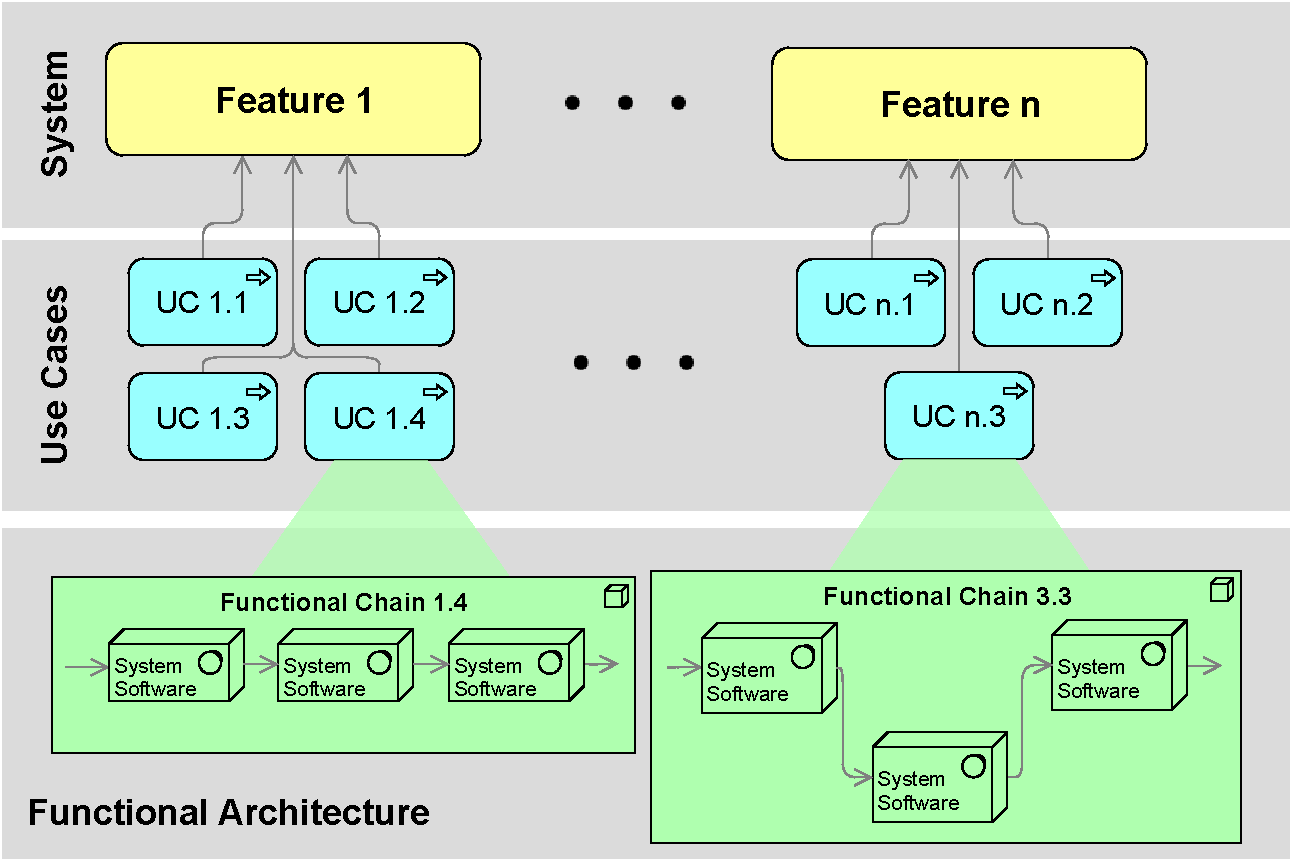
\includegraphics[width=\linewidth]{SchemaChaineFonctionnelle.pdf}
			\caption{Définition d'architecture fonctionnelle}
			\label{fig:funcArch}
		\end{figure}
	
		Il faut considérer les chaînes de tâches comme une implémentation d'une fonctionnalité système, qui va de son déclenchement jusqu'à sa terminaison. Cela correspond une majeure partie du temps à une chaîne de réaction allant d'une donnée d'entrée (détection d'un capteur par exemple) jusqu'à la conséquence (activation d'un actionneur), en passant par un algorithme de décision. Il s'agit donc d'un modèle classique de type Sense-Compute--Control où en pratique le Compute est implémenté par une Chaîne de tâches.
		Comme on l'a vu en début de ce Chapitre, il n'est pas tout à fait pertinent d'associer directement des niveaux de criticités au sens des standards logiciels de Sûreté de Fonctionnement (ASIL D à ASIL A et QM pour ISO 26262 en automobile typiquement), aux niveaux de criticités pour l'Agent de Surveillance et de Contrôle. Le seul lien qu'il est possible de déduire de la classification ASIL étant plutôt qu'il est improbable que les tâches de la chaîne critique soient de niveau QM. Les tâches de niveau d'ASIL élevé (ASIL D au maximum) feront certainement part de la chaîne de tâches critiques, mais il est difficile à partir d'un niveau d'ASIL plus faible d'en déduire le niveau d'importance d'une tâche. 
		Ce critère d'importance est crucial étant donné que les tâches non critiques du système pourront être mises en pause par l'agent de Surveillance et Contrôle.
		
	
		Si l'on revient au cas d'application automobile, les spécifications sont données par étapes. Dans un premier temps, il y a la spécification Système, qui liste la totalité des fonctionnalités (\emph{Features}) qui doivent être embarquées. Chaque Feature contient un certain nombre de Cas d'Utilisation (\emph{Use Cases}), qui se définissent par un scénario de fonctionnement et le comportement attendu de la fonctionnalité. Enfin, pour chaque Use Case, il est possible de représenter la Chaîne Fonctionnelle qui définit les blocs logiciels qui sont mobilisés pour réaliser ce cas d'utilisation. L'ensemble de ces chaînes constitue l'architecture fonctionnelle du système. Ces différentes couches de spécification système sont représentées dans la~\autoref{fig:funcArch}. %Si l'on va encore plus en détail dans la spécification, il y aurait ensuite l'allocation physique des blocs logiciels...


		Cette façon de modéliser le système semble être adaptée à notre approche pour identifier la méthode de sélection des tâches critiques, ainsi que quel type de spécification prendre en compte pour l'échéance d'exécution bout-en-bout, qui sont des données déjà existantes au niveau de l'architecture fonctionnelle. Une fois la chaîne fonctionnelle déterminée en fonction du système étudié, il est alors possible de descendre jusqu'à la spécification des tâches logicielles qui découlent de cette architecture pour identifier les tâches critiques et non critiques.
		
\cmnt{
		\comment{A FAIRE}{Je pensais aborder dans cette section ce qui est repris ci-dessous en anglais, avec le lien entre les spécifications côté industrie et le choix de la chaîne de tâche. Mais au final ça fait beaucoup doublon avec ce que j'ai mis en début de chapitre, "Notion de criticité". Du coup je ne suis pas sûr de comment agencer tout ça. Et de voir comment j'inscris cette partie avec peut-être le fait de parler d'AUTOSAR / Adaptive AUTOSAR et ARINC 653...}
		% A critical task chain must describe the implementation of a system functionality from its triggering to its consequence. This would stick most of the time with a computing chain going from a sensor measure to an actuator command. First idea would be to stick with safety criticality levels (ASIL D to ASIL A and QM, for automotive applications), but we quickly notice that there is no direct link between this classification and critical tasks chains. A safety critical task is not necessarily defined from its timing constraints. The only possible conclusion here is that a critical task chain only includes non-QM tasks. 
		\smallbreak
		We propose here a definition based around high-level specifications as represented in figure~\ref{fig:funcArch}. The global system is defined as a set of features\footnote{Features: all the services the system must provide. e.g: Lane Support System (LSS) is a feature.}. Every feature gathers a set of functionalities that are translated into Use Cases\footnote{e.g: Lane Departure Warning \& Lane Keeping Assist are part of the use cases of LSS feature.}. A Use Case defines a feature behavior for a given context and inputs (and the consequent outputs). Finally, those are translated into functional chains representing different functions and their interactions needed for the realization of the Use Case. 


            
		If we combine this information with a severity classification in case of failure of the use cases, it is possible to define critical chains as functional chains with a high severity risk. This is one possible criterion allowing an easy separation between a critical functional chain and the others. It could be adapted during the design phase, depending on the functional chains allocated to the processor. 
		\smallbreak
		Such information allows to define the software components involved in the critical task chain. All the software components used to realize a critical functional chain form a critical task chain at an OS point of view. At this point, it is possible to define the task chain end-to-end deadline, following the severity temporal risk in case of failure. Such deadline should be at minimum the sum of individual tasks deadline, but could probably be higher, depending on the global system and the task chain function. Our objective is to guarantee such critical task chain end-to-end execution time on the multicore.
	}
		
\ifdefined\included
\else
\bibliographystyle{StyleThese}
\bibliography{these}
\end{document}
\fi
